\section{策略梯度}
本章开始介绍基于策略梯度(policy based)的算法,与前面介绍的基于价值(value based)的算法(包括Q learning,SARSA以及DQN等等)不同,这类算法直接对策略本身进行近似优化。在这种情况下,我们可以将策略描述成一个带有参数$\theta$的连续函数,该函数将某个状态作为输入,输出的不再是某个确定性(deterministic)的离散动作,而是对应的动作概率分布,通常用$\pi_{\theta}(a|s)$表示,称作随机性(stochastic)策略。下面我们将从最基本的策略梯度算法展开。

\subsection{策略梯度算法}

尽管策略梯度算法是将策略参数化成一个连续的函数$\pi_{\theta}(a|s)$,但是与基于价值的算法本质上是一样的,最终的优化目标都是累积的价值期望$V^{*}(s)$。例如在前面章节的 Q learning 算法中,我们利用贝尔曼方程求解马尔科夫决策过程中的最佳决策序列,进而求出对应的最优动作价值函数$Q^{*}(s,a)$,不清楚的读者可以再回到前面的内容温习一下。

策略一般记作 $\pi$。假设我们使用深度学习来做强化学习,策略就是一个网络。网络里面有一些参数,我们用 $\theta$ 来代表 $\pi$ 的参数。
网络的输入是智能体看到的东西,如果让智能体玩视频游戏,智能体看到的东西就是游戏的画面。智能体看到的东西会影响我们训练的效果。例如,在玩游戏的时候, 也许我们觉得游戏的画面是前后相关的,所以应该让策略去看从游戏开始到当前这个时间点之间所有画面的总和。因此我们可能会觉得要用到循环神经网络(recurrent neural network,RNN)来处理它,不过这样会比较难处理。
我们可以用向量或矩阵来表示智能体的观测,并将观测输入策略网络,策略网络就会输出智能体要采取的动作。
\figref{fig:actor_policy} 就是具体的例子,策略是一个网络;输入是游戏的画面,它通常是由像素组成的;输出是我们可以执行的动作,有几个动作,输出层就有几个神经元。假设我们现在可以执行的动作有 3 个,输出层就有 3 个神经元,每个神经元对应一个可以采取的动作。输入一个东西后,网络会给每一个可以采取的动作一个分数。我们可以把这个分数当作概率,演员根据概率的分布来决定它要采取的动作,比如 0.7 的概率向左走、0.2 的概率向右走、0.1的概率开火等。概率分布不同,演员采取的动作就会不一样。

\begin{figure}[hbt]
    \centering
    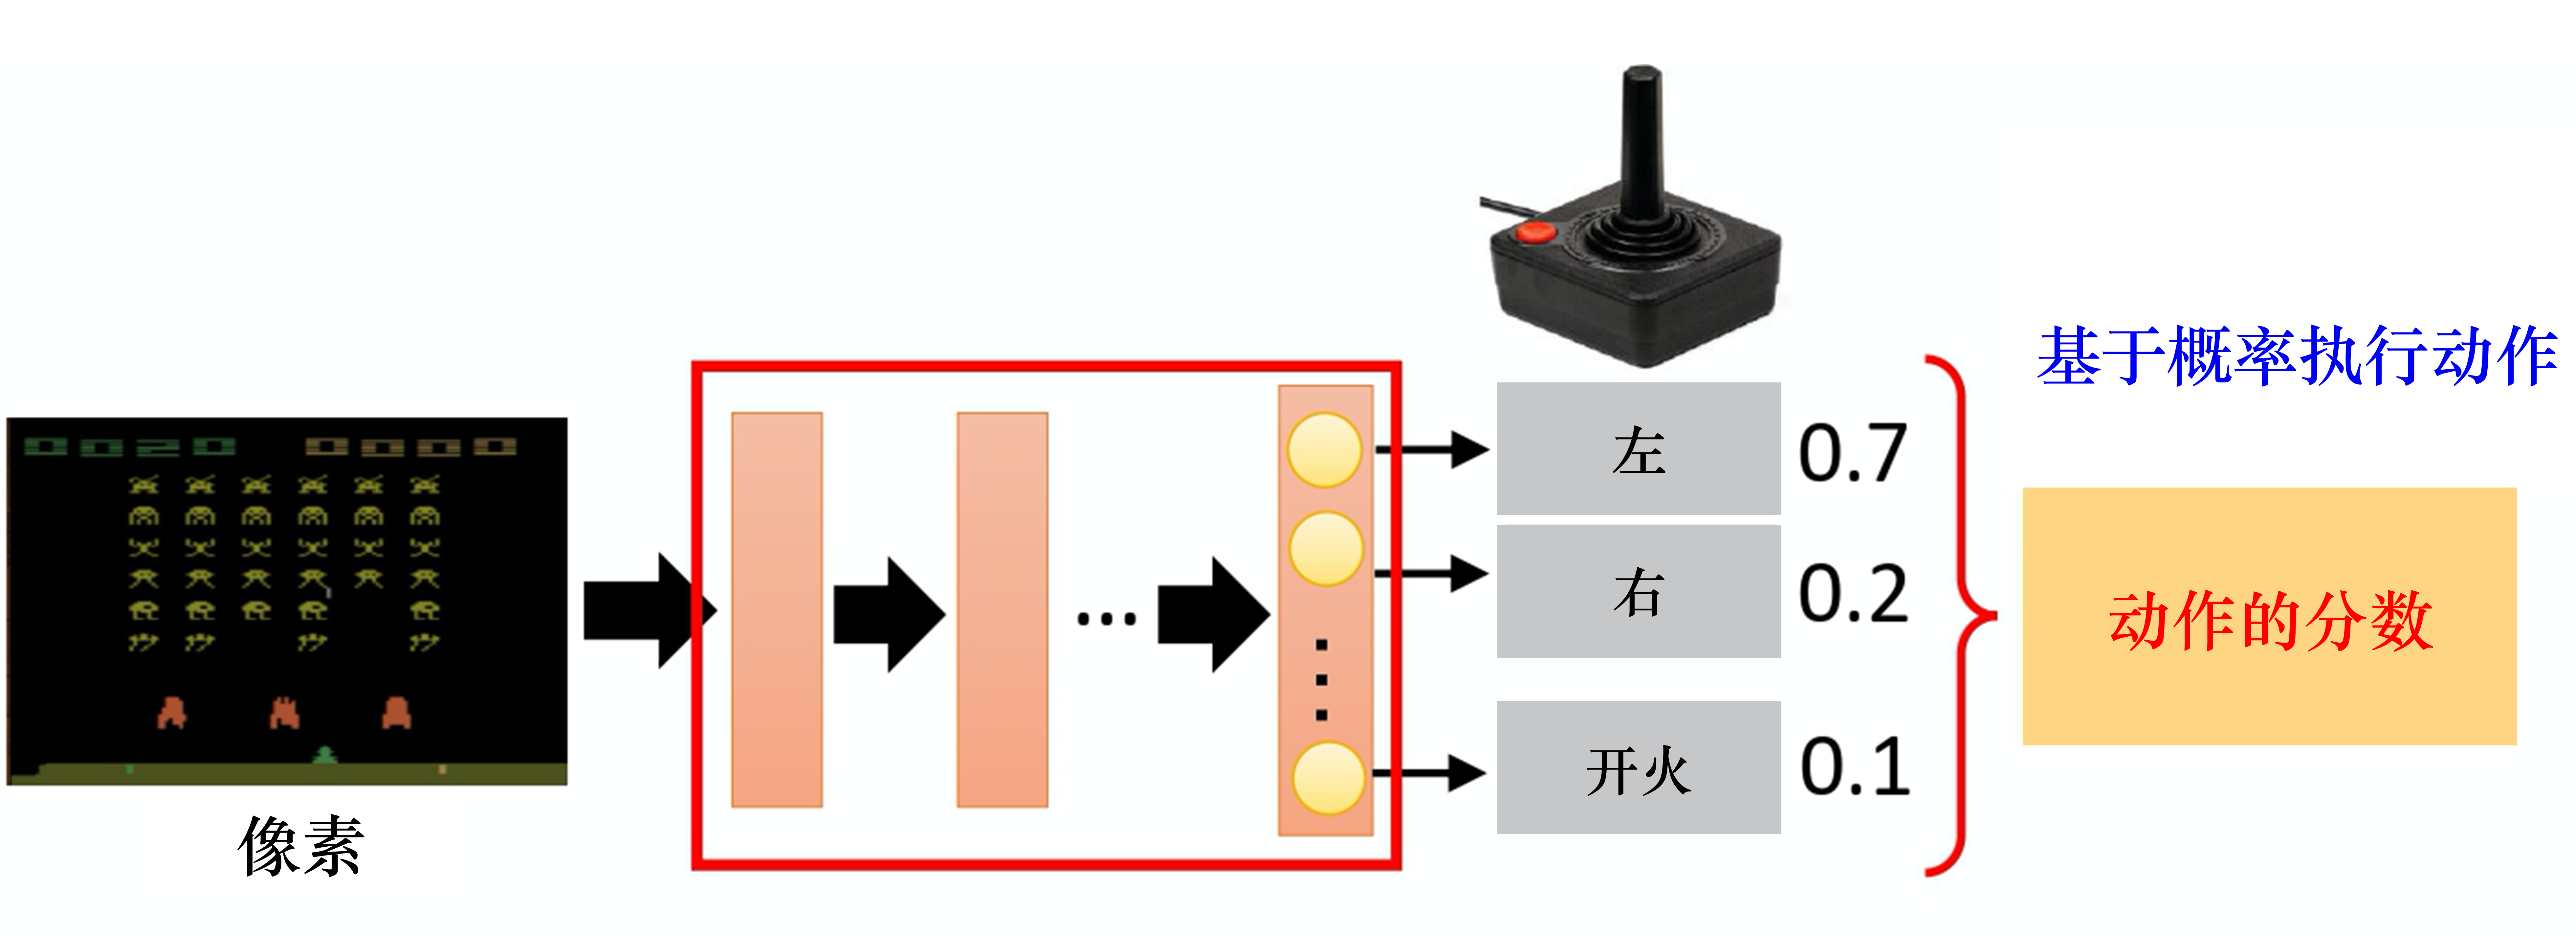
\includegraphics[width=0.5\linewidth]{ch6/figs/actor_policy.png}
    \caption{演员的策略}
    \label{fig:actor_policy}
\end{figure}

接下来我们用一个例子来说明演员与环境交互的过程。

如\figref{fig:example_play_game}所示,首先演员会看到一个视频游戏的初始画面,接下来它会根据内部的网络(内部的策略)来决定一个动作。假设演员现在决定的动作是向右,决定完动作以后,它就会得到一个奖励,奖励代表它采取这个动作以后得到的分数。

我们把游戏初始的画面记作 $s_0$, 把第一次执行的动作记作 $a_0$,把第一次执行动作以后得到的奖励记作 $r_1$。
这里不同的人有不同的记法,有人觉得应该从 $s_1$ 开始,并且执行 $a_1$ 得到的奖励应该记为 $r_1$,这两种记法都可以。只是一般来说,是智能体先做出动作,然后环境再输出奖励和新的状态,也就是说这个新的状态和奖励应该对应着同一时刻,也就是同一下标。我们通常喜欢从 0 时刻开始记录轨迹,此轨迹可以将交互过程清晰地体现出来。
演员决定一个动作以后,就会看到一个新的游戏画面$s_1$。把 $s_1$ 输入给演员,演员决定要开火,它可能打败了一只怪兽,就得到五分。这个过程反复地持续下去,直到在某一个时间点执行某一个动作,得到奖励之后,环境决定这个游戏结束。例如,如果在这个游戏里面,我们控制宇宙飞船去击杀怪兽,如果宇宙飞船被毁或是把所有的怪兽都清空,游戏就结束了。

\begin{figure}[hbt]
    \centering
    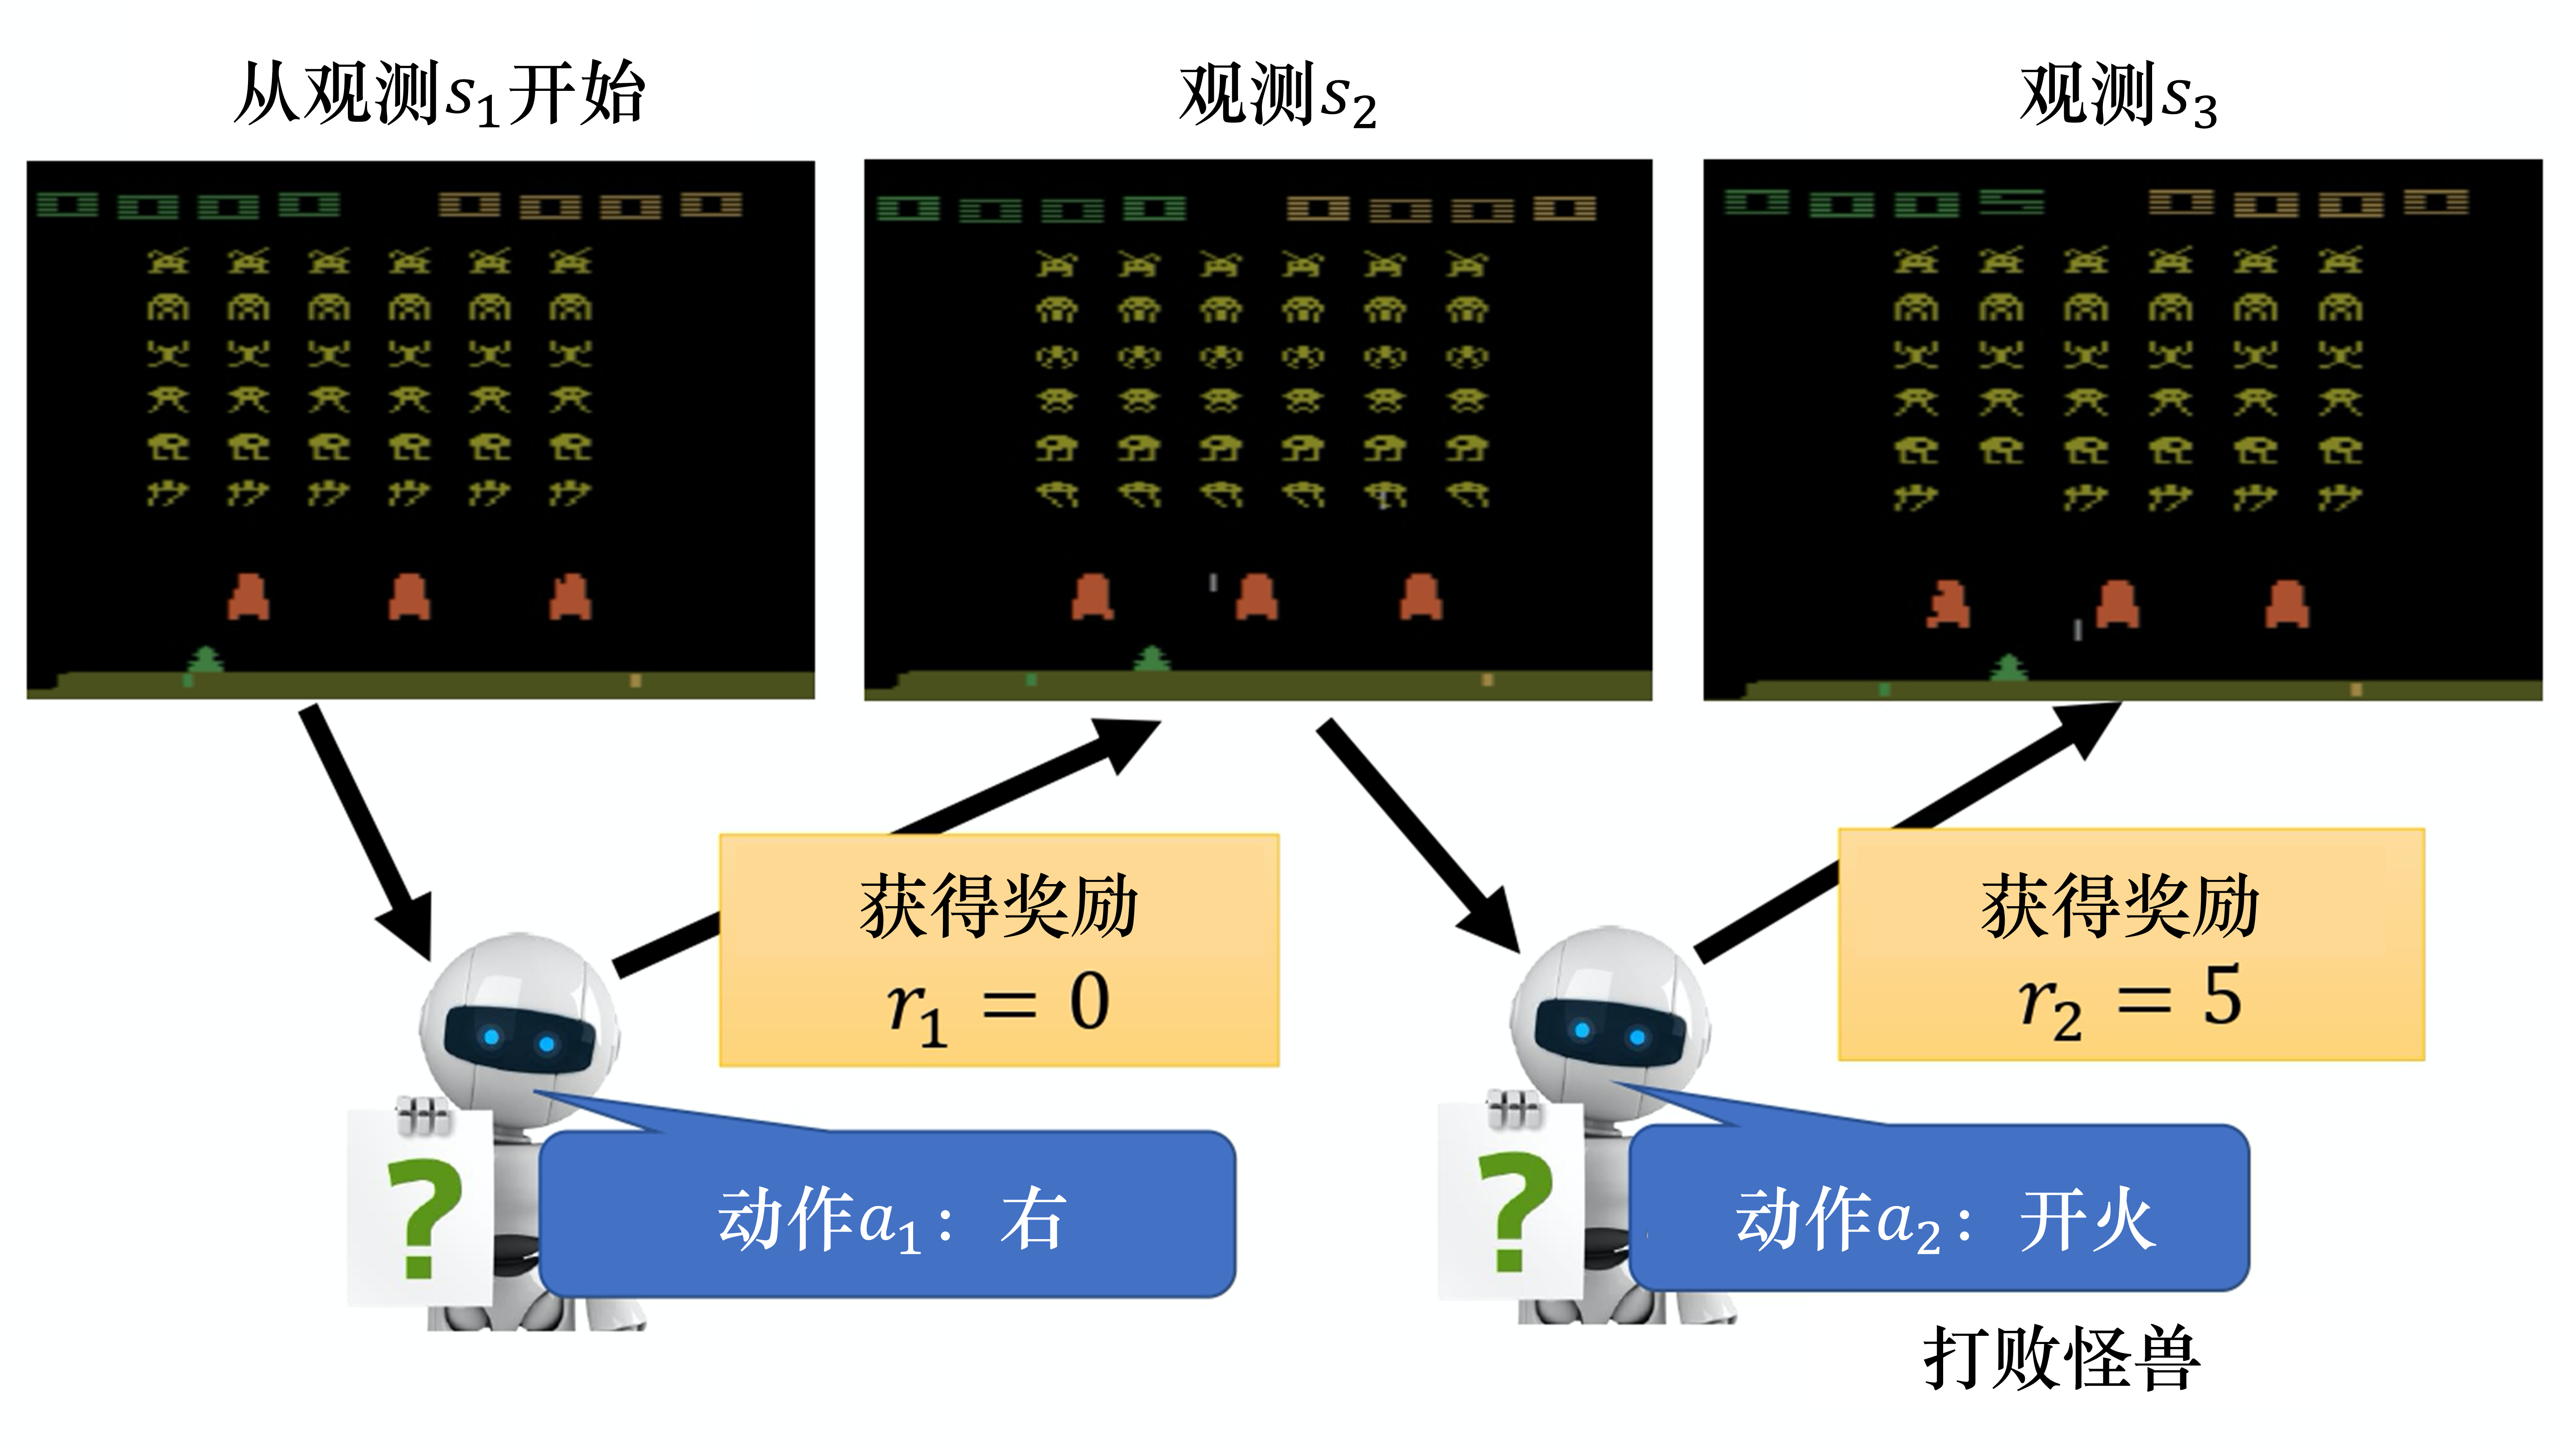
\includegraphics[width=0.5\linewidth]{ch6/figs/example_play_game.png}
    \caption{玩视频游戏的例子}
    \label{fig:example_play_game}
\end{figure}


那么在策略梯度算法中我们怎样去推导出最优策略下的价值期望呢?首先我们知道强化学习解决的问题基本上都可以被描述为马尔可夫决策过程,而马尔可夫决策过程同时也是成环境与智能体不断交互的过程,即环境与策略不断交互的过程,因为智能体是策略的载体。如\figref{fig:env_agent} 所示,环境首先“吐”出一个初始状态$s_0$,然后智能体观测到状态$s_0$,它会“吐”出相应的动作 $a_0$。紧接着环境接收到 $a_0$ 反馈出新的状态 $s_1$,然后智能体观测到新的状态继续采取新的动作......如此循环往复,直到满足环境的停止条件为止。

\begin{figure}[hbt]
    \centering
    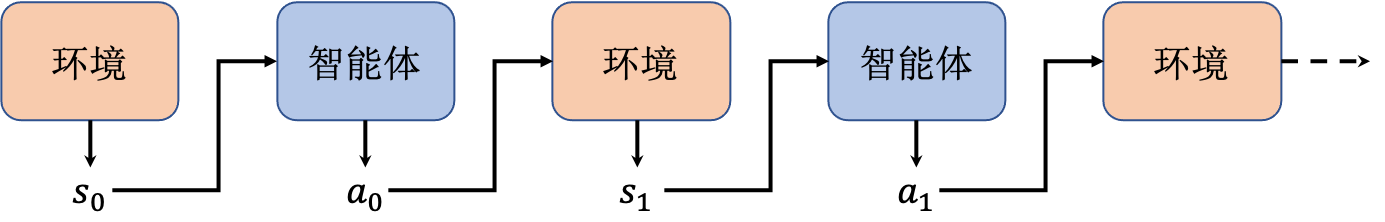
\includegraphics[width=0.5\linewidth]{ch6/figs/env_agent.png}
    \caption{智能体与环境}
    \label{fig:env_agent}
\end{figure}

在这样一个过程之后,我们把环境输出的所有状态 $s$ 与智能体输出的对应动作 $a$ 全部组合起来,就形成了一条轨迹(trajectory),即
\begin{equation}
    \label{eq:}
    \tau=\left\{s_{0}, a_{0}, s_{1}, a_{1}, \cdots, s_{t}, a_{t}\right\}
\end{equation}

这里环境也可以看作一个函数,我们设在给定状态$s_t$和动作$a_t$的情况下,它“吐”出状态$s_{t+1}$的概率为$p(s_{t+1} | s_{t}, a_{t})$,即是马尔可夫决策过程中的转移概率。此外我们假设环境以一个概率$p(s_{0})$“吐”出初始状态,在给定策略函数$\pi_{\theta}(a|s)$的情况下,我们就可以计算某个轨迹$\tau$发生的概率为
\begin{equation}
    \label{eq:station_dist}
    \begin{aligned}
        P_{\theta}(\tau)
        &=p(s_{0}) \pi_{\theta}(a_{0} | s_{0}) p(s_{1} | s_{0}, a_{0}) \pi_{\theta}(a_{1} | s_{1}) p(s_{2} | s_{1}, a_{1}) \cdots \\
        &=p(s_{0}) \prod_{t=0}^{T} \pi_{\theta}\left(a_{t} | s_{t}\right) p\left(s_{t+1} | s_{t}, a_{t}\right)
    \end{aligned}
\end{equation}

也就是说我们先计算环境输出初始状态 $s_0$ 的概率 $p(s_0)$,再计算智能体根据 $s_0$ 动作执行 $a_0$ 的概率,也就是策略函数$p_{\theta}\left(a_{0} | s_{0}\right)$。然后环境结合当前状态$s_0$根据动作$a_0$以一定的概率反馈出新的状态 $s_1$,也就是转移概率$p(s_{1} | s_{0}, a_{0})$。 
这样的转移概率通常情况下是一定存在的,也就是不为0,因为 $s_1$ 与 $s_0$ 一般说来是有关系的。举个例子,我们玩电脑游戏时,一般都是根据每一帧的游戏画面给出的信息来采取我们认为的最优动作以便于获得游戏的最终胜利。这种情况下,游戏画面可以看作状态,比如当前帧画面为$s_0$,下一帧画面就是 $s_1$ 。由于游戏画面是连续的,因此下一帧游戏画面$s_1$ 与上一帧游戏画面$s_0$ 通常是有联系的。如果显示器输出游戏画面的时候没有概率,极端情况下游戏的画面就会始终停留在某一帧下,此时我们只要找到一条路径就可以过关了,这样的游戏就没有意义。所以输出游戏画面时通常有一定概率,给定同样的前一个画面,我们采取同样的动作,下次产生的画面不一定是一样的。如此反复执行下去,我们就可以计算出一条轨迹 $\tau$ 出现的概率了。

前面讲到,无论是基于价值还是基于策略梯度的方法,我们的目标都是希望最终累积的价值期望最大,这个价值的定义或者说近似也是比较多样的,可以是简单的累积奖励之和,也可以是包含折扣因子$\gamma$的累积奖励之和,也就是通常我们所说的回报$G$(return)。如何近似这个价值期望也是研究者们近年来一直在不断地优化策略梯度算法的重点之一,这个在后面章节我们讲A2C和GAE等算法的时候会继续展开,现在我们姑且将这个价值近似为最为简单的累积奖励。

再简单回顾一下马尔可夫决策过程。我们知道强化学习中除了智能体和环境之外,还会涉及奖励。奖励一般是由环境反馈得到的,如\figref{fig:expected_reward} 所示,环境根据在某个状态以及在这一状态下智能体采取的某个动作来决定这个动作可以得到的分数,也就是奖励。例如,输入$s_0$、$a_0$,它会输出$r_1$;输入 $s_1$、$a_1$,会输出 $r_2$ 等等,如\eqref{eq:traj_reward}。

\begin{equation}
    \label{eq:traj_reward}
    \tau=\left\{s_{0}, a_{0}, s_{1},r_{1},a_{1},\cdots, s_{t-1}, r_{t-1}, a_{t-1},s_{t},r_{t}\right\}
\end{equation}

\begin{figure}[hbt]
    \centering
    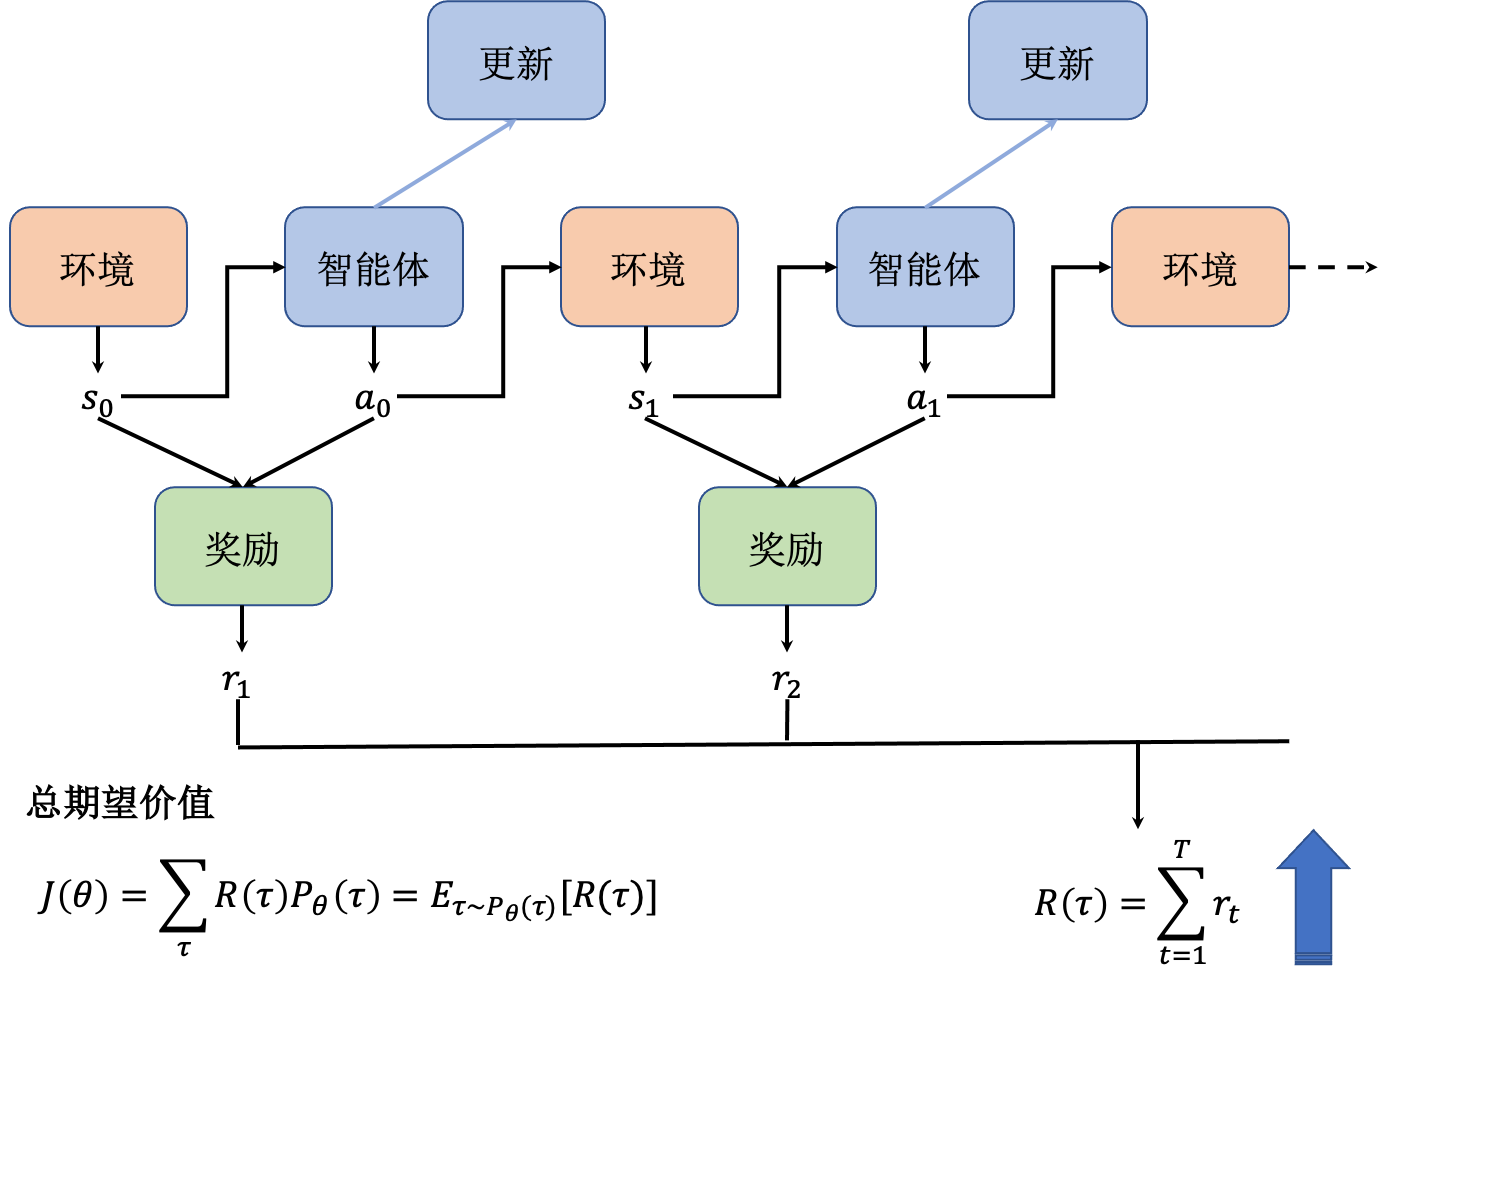
\includegraphics[width=0.5\linewidth]{ch6/figs/expected_reward.png}
    \caption{期望的奖励}
    \label{fig:expected_reward}
\end{figure}

奖励一般也可以近似成关于状态和动作的函数,即$r_{t+1}=r(s_t,a_t),t=0,1,\cdots$。对于一条轨迹$\tau$,我们可以计算其对应的累积奖励为$R(\tau)=\sum_{t=0}^T r\left(s_t, a_t\right)$。那么在给定的策略下,即参数$\theta$固定,对于不同的初始状态,会形成不同的轨迹$\tau_{1},\tau_{2},\cdots$,对应轨迹的出现概率前面已经推导出来为$P_{\theta}(\tau_{1}),P_{\theta}(\tau_{2}),\cdots$,累积奖励则为$R(\tau_{1}),R(\tau_{2}),\cdots$。回忆一下概率论中的全期望公式,是不是该策略的价值期望公式就可以通过每条轨迹的概率乘上对应的累积奖励再求和得到呢?答案是肯定的!如\eqref{eq:expect_policy},这就是我们所要找的目标函数。

\begin{equation}
    \label{eq:expect_policy}
    \begin{aligned}
    J(\pi_{\theta}) = P_{\theta}(\tau_{1})R(\tau_{1})+P_{\theta}(\tau_{2})R(\tau_{2})+\cdots \\
    &=\int_\tau P_{\theta}(\tau) R(\tau) \\ 
    &=E_{\tau \sim P_\theta(\tau)}[\sum_t r(s_t, a_t)] \\
    &=\underset{\tau \sim \pi_\theta}{E}[R(\tau)] 
    \end{aligned}
\end{equation}

有了目标函数,读者如果学过深度学习就会很自然地想到用梯度下降或者上升的方法来求解对应的最优参数$\theta^{*}$,这里需要用到梯度上升法,因为我们的目标是让总的累积价值期望$J(\pi_{\theta})$最大,而不是最小。当然我们也可以将目标函数取负号,即求解$-J(\pi_{\theta})$,然后再用梯度下降法去求解。梯度下降是更为普遍的做法,熟悉Tensorflow或者PyTorch等框架的读者应该比较清楚,这些框架默认的优化器设置就是梯度下降的,因此实际编程的时候如果我们的目标是最大化某个量,我们就会取这个量的相反数来优化。再比如用过scipy模块中的linprog函数来求解线性规划的读者也会知道,linprog函数默认的设置是求目标函数的最小值,而不是最大值,当我们的实际问题是求最大值时,我们也会进行取反的操作。

回归正题,梯度下降方法的关键还是在于求出$J(\pi_{\theta})=\int_\tau P_{\theta}(\tau) R(\tau)$的梯度,但是一眼看上去似乎不太好求。我们先不着急,首先我们是求关于参数$\theta$的梯度,可以看到$R(\tau)$跟$\theta$其实是没有关联的,因此在求解梯度的时候可以将这一项看作常数。那么接下来就是怎么求$P_{\theta}(\tau)$关于$\theta$的梯度了,我们需要用到一个对数微分的技巧,即$\log x$的导数是$1/x$。注意这里我们通常默认$\log$的底数是$e$,因此这里$\log x$也就是我们常见的$\ln x$,在大学数学之后的概念中我们通常是写作$\log x$,同学们请务必习惯。根据这个技巧,我们就可以推出\eqref{eq:log_trick}。
\begin{equation}
    \label{eq:log_trick}
    \nabla_\theta P_{\theta}(\tau)= P_{\theta}(\tau) \frac{\nabla_\theta P_{\theta}(\tau)}{P_{\theta}(\tau) }= P_{\theta}(\tau) \nabla_\theta \log P_{\theta}(\tau)
\end{equation}

现在的问题就从求$P_{\theta}(\tau)$的梯度变成了求$\log P_{\theta}(\tau)$的梯度了,即求$\nabla_\theta \log P_{\theta}(\tau)$。我们先求出$\log P_{\theta}(\tau)$,根据\eqref{eq:station_dist},$P_{\theta}(\tau)=p(s_{0}) \prod_{t=0}^{T} \pi_{\theta}\left(a_{t} | s_{t}\right) p\left(s_{t+1}  s_{t}, a_{t}\right)$,再根据对数公式$log (ab) = log a + log b$,即可求出:

\begin{equation}
    \label{eq:station_dist_log}
    \log P_{\theta}(\tau)= \log p(s_{0})  +  \sum_{t=0}^T(\log \pi_{\theta}(a_t \mid s_t)+\log p(s_{t+1} \mid s_t,a_t))
\end{equation}

我们惊奇地发现$\log P_{\theta}(\tau)$展开之后只有中间的项$\log \pi_{\theta}(a_t \mid s_t)$跟参数$\theta$有关,也就是说其他项关于$\theta$的梯度为0,如\eqref{eq:station_dist_log_grad}所示。
\begin{equation}
    \label{eq:station_dist_log_grad}
    \begin{aligned}
    \nabla_\theta \log P_{\theta}(\tau) &=\nabla_\theta \log \rho_0\left(s_0\right)+\sum_{t=0}^T\left(\nabla_\theta \log \pi_\theta\left(a_t \mid s_t\right)+\nabla_\theta \log p\left(s_{t+1} \mid s_t, a_t\right)\right) \\
    &=0+\sum_{t=0}^T\left(\nabla_\theta \log \pi_\theta\left(a_t \mid s_t\right)+0\right) \\
    &=\sum_{t=0}^T \nabla_\theta \log \pi_\theta\left(a_t \mid s_t\right)
    \end{aligned}
\end{equation}

现在我们就可以很方便地求出目标函数的梯度了,如\eqref{eq:pg_ob_grad}所示。

\begin{equation}
    \label{eq:pg_ob_grad}
    \begin{aligned}
    \nabla_\theta J\left(\pi_\theta\right) &=\nabla_\theta \underset{\tau \sim \pi_\theta}{\mathrm{E}}[R(\tau)] \\
    &=\nabla_\theta \int_\tau P_{\theta}(\tau) R(\tau) \\
    &=\int_\tau \nabla_\theta P_{\theta}(\tau) R(\tau) \\
    &=\int_\tau P_{\theta}(\tau) \nabla_\theta \log P_{\theta}(\tau) R(\tau) \\
    &=\underset{\tau \sim \pi_\theta}{\mathrm{E}}\left[\nabla_\theta \log P_{\theta}(\tau) R(\tau)\right]\\
    &= \underset{\tau \sim \pi_\theta}{\mathrm{E}}\left[\sum_{t=0}^T \nabla_\theta \log \pi_\theta\left(a_t \mid s_t\right) R(\tau)\right]
    \end{aligned}
\end{equation}

我们再简单解释一下\eqref{eq:pg_ob_grad}中的步骤,首先第一行就是目标函数的表达形式,到第二行就是全期望展开式,到第三行就是利用了积分的梯度性质,即梯度可以放到积分号的里面也就是被积函数中,第四行到最后就是对数微分技巧了。回过头来看下,我们为什么要用到对数微分技巧呢?这其实是一个常见的数学技巧:当我们看到公式中出现累乘的项时,我们通常都会取对数简化,因为根据对数公式的性质可以将累乘的项转换成累加的项,这样一来问题会更加便于处理。

我们可以直观地理解\eqref{eq:pg_ob_grad},即在采样到的数据里面,$(s_t,a_t)$ 可看作整个轨迹 $\tau$ 里面的某一个状态$-$动作对,假设我们在 $s_t$ 下执行 $a_t$时,最后发现 $\tau$ 的奖励是正的,我们就要增加在 $s_t$ 下执行 $a_t$ 的概率。反之,如果若 $\tau$ 的奖励是负的, 我们就要减少在 $s_t$ 下执行 $a_t$ 的概率,这其实就是梯度的思想。前面讲到我们将目标函数取反,就可以用梯度下降方法求取最优的参数$\theta$,即
\begin{equation}
    \label{eq:theta_update}
    \theta \leftarrow \theta - \alpha (-\nabla_\theta J\left(\pi_\theta\right))
\end{equation}
其中$\alpha$表示学习率,不明白\eqref{eq:theta_update}的读者就可以再去温习一下梯度下降法的原理,实际编程过程中我们还可以用 Adam、RMSProp 等方法来调整学习率,具体见后面的实战内容。

\subsection{REINFORCE算法}

在本小节中我们将介绍策略梯度中最简单也是最经典的一个算法\kw{REINFORCE},又称蒙特卡洛策略梯度算法(Monte Carlo Policy Gradient)。在介绍该算法之前,我们先回顾一下蒙特卡洛方法。

如\figref{fig:mc_td} 所示,蒙特卡洛方法可以理解为算法完成一个回合之后,再利用这个回合的数据去更新策略,也就是学习。因为我们已经获得了整个回合的数据,相应地也能够知道每一个步骤的奖励,我们可以很方便地计算每个步骤的未来总奖励,即回报 $G_t$。$G_t$ 是未来总奖励,代表从这个步骤开始,我们能获得的奖励之和。$G_1 $代表我们从第一步开始,往后能够获得的总奖励。$G_2$ 代表从第二步开始,往后能够获得的总奖励。

相比蒙特卡洛方法一个回合更新一次,时序差分方法是每个步骤更新一次,即每走一步,更新一次,时序差分方法的更新频率更高。时序差分方法使用Q函数来近似地表示未来总奖励 $G_t$。
\begin{figure}[hbt]
    \centering
    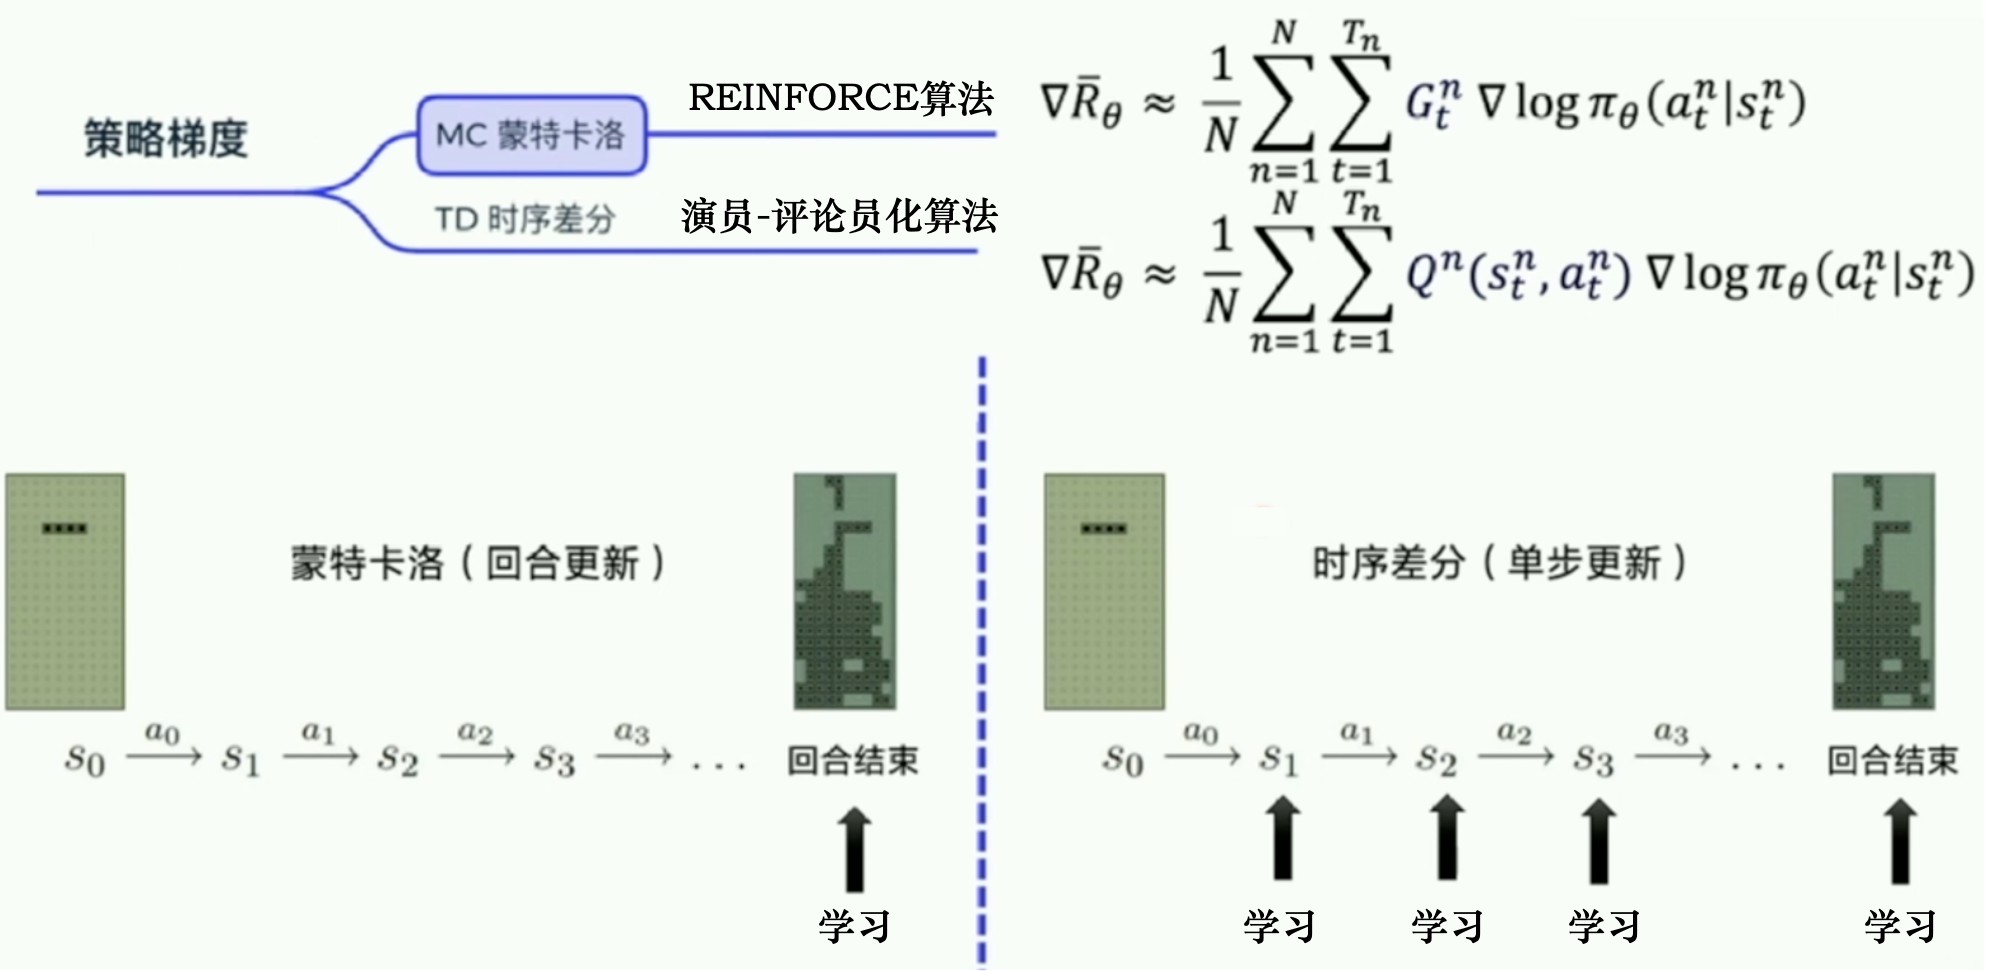
\includegraphics[width=0.5\linewidth]{ch6/figs/mc_td.png}
    \caption{蒙特卡洛方法与时序差分方法}
    \label{fig:mc_td}
\end{figure}

REINFORCE 算法正是利用蒙特卡洛算法来计算每回合生成的轨迹的价值,即$G_t$,然后乘上对应轨迹的概率从而计算总的价值期望,即\eqref{eq:reinforce_update}。

\begin{equation}
    \label{eq:reinforce_update}
    \nabla J_{\theta} \approx \frac{1}{N} \sum_{n=1}^{N} \sum_{t=1}^{T_{n}} G_{t}^{n} \nabla \log \pi_{\theta}\left(a_{t}^{n} \mid s_{t}^{n}\right)
\end{equation}

我们回顾一下前面策略梯度基础推导中以轨迹为对象的公式,即\eqref{eq:pg_ob_grad_2},如下:

\begin{equation}
    \begin{aligned}
    \nabla_\theta J\left(\pi_\theta\right) = \underset{\tau \sim \pi_\theta}{\mathrm{E}}\left[\sum_{t=0}^T \nabla_\theta \log \pi_\theta\left(a_t \mid s_t\right) R(\tau)\right]
    \end{aligned}
\end{equation}

其实这跟 REINFORCE 算法的目标函数梯度公式 (\eqref{eq:reinforce_update})几乎是等效的,换句话说,REINFORCE 算法本质上就是计算轨迹的概率和对应轨迹的累积价值然后得到总的价值期望,是一种比较纯的原始的策略梯度算法。前面我们讲到计算轨迹对应的奖励是十分繁琐的,因为我们不确定要计算多少步。但是 REINFORCE 算法这里与前面策略梯度基础推导公式不同的是,它使用了带有折扣因子$\gamma$的回报$G_t$来代替单纯的累积奖励$R(\tau)$去近似对应轨迹的累积奖励。在之前关于贝尔曼公式的推导中,我们其实已经领教过了这种带折扣因子的魅力。这种折扣因子可以让当前时刻和下一时刻的价值很好地联系起来,从而避免无限循环状态下的计算问题,即$V_t = r_{r+1}+\gamma V_{t+1}$,从而能够很方便地进行后面的推导。这里的回报$G_t$同理,如\eqref{eq:future_relation}。
\begin{equation}
    \label{eq:future_relation}
    \begin{aligned}
        G_{t} &=\sum_{k=t+1}^{T} \gamma^{k-t-1} r_{k} \\
        &=r_{t+1}+\gamma G_{t+1}
        \end{aligned}
\end{equation}

建立起了这样一种联系之后,在数学分析或编写代码上,我们是从后往前推,即从$G_T$一步一步地往前推到$G_1$。相比于原来每个轨迹都要从头开始计算对应的$R(\tau)$,已经在简化的道路上迈出了不小的一步了。

梯度公式弄清楚之后,我们就可以直接写出对应的伪代码了。如\figref{fig:REINFORCE} 所示,
REINFORCE 的伪代码主要看最后4行,先产生一个回合的数据,比如 
$$
(s_1,a_1,G_1),(s_2,a_2,G_2),\cdots,(s_T,a_T,G_T)
$$
然后针对每个动作计算梯度 $\nabla \ln \pi(a_t|s_t,\theta)$ 。在代码中,我们要获取神经网络的输出。神经网络会输出每个动作对应的概率值(比如0.2、0.5、0.3),然后我们还可以获取实际的动作$a_t$,并转成独热(one-hot)向量(比如[0,1,0])与 $\log ([0.2,0.5,0.3])$ 相乘就可以得到 $\ln \pi(a_t|s_t,\theta)$  。
\begin{figure}[hbt]
    \centering
    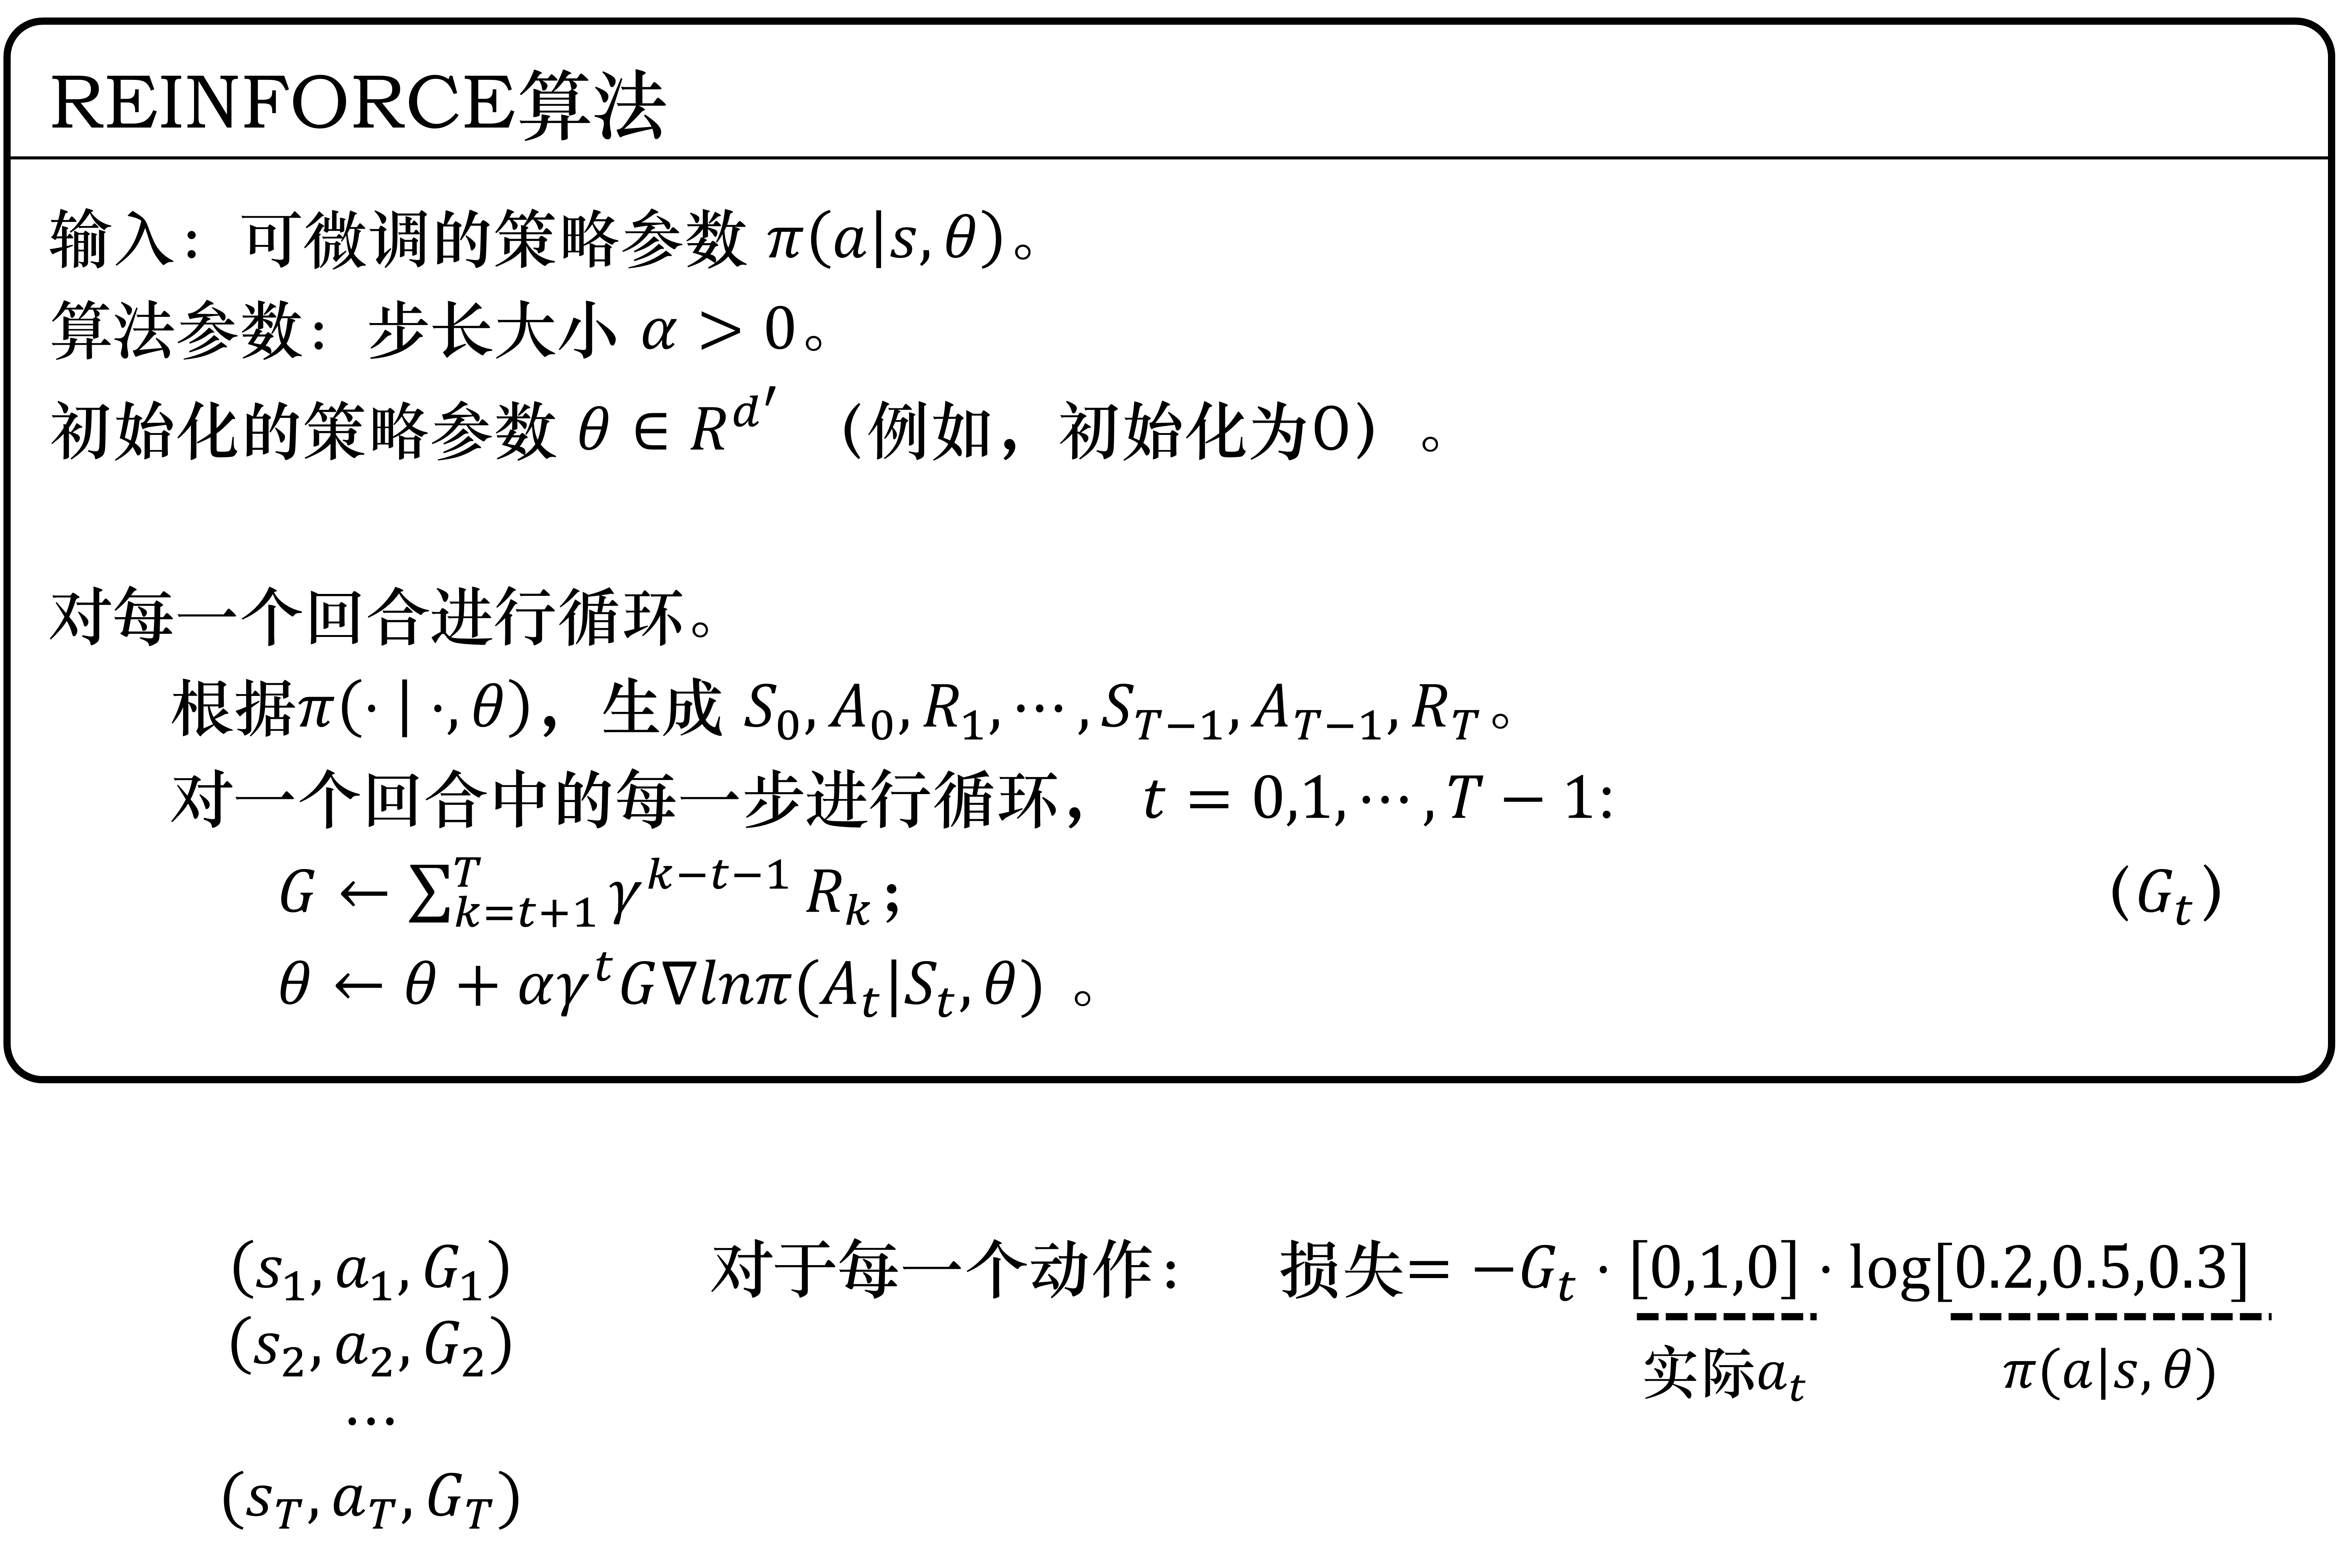
\includegraphics[width=0.5\linewidth]{ch6/figs/REINFORCE.png}
    \caption{REINFORCE算法}
    \label{fig:REINFORCE}
\end{figure}

\begin{tcolorbox}[colframe=blue!25,colback=blue!10]
独热编码(one-hot encoding)通常用于处理类别间不具有大小关系的特征。 例如血型,一共有4个取值(A型、B型、AB型、O型),独热编码会把血型变成一个4维稀疏向量,A型血表示为$[1,0,0,0]$,B型血表示为$[0,1,0,0]$,AB型血表示为$[0,0,1,0]$,O型血表示为$[0,0,0,1]$,\upcite{zhugesheng}。
\end{tcolorbox}

如\figref{fig:mnist_recognition} 所示,
手写数字识别是一个经典的多分类问题,输入是一张手写数字的图片,经过神经网络处理后,输出的是各个类别的概率。我们希望输出的概率分布尽可能地贴近真实值的概率分布。
因为真实值只有一个数字 9,所以如果我们用独热向量的形式给它编码,也可以把真实值理解为一个概率分布,9 的概率就是1,其他数字的概率就是 0。
神经网络的输出一开始可能会比较平均,通过不断地迭代、训练优化之后,我们会希望输出9 的概率可以远高于输出其他数字的概率。

\begin{figure}[hbt]
    \centering
    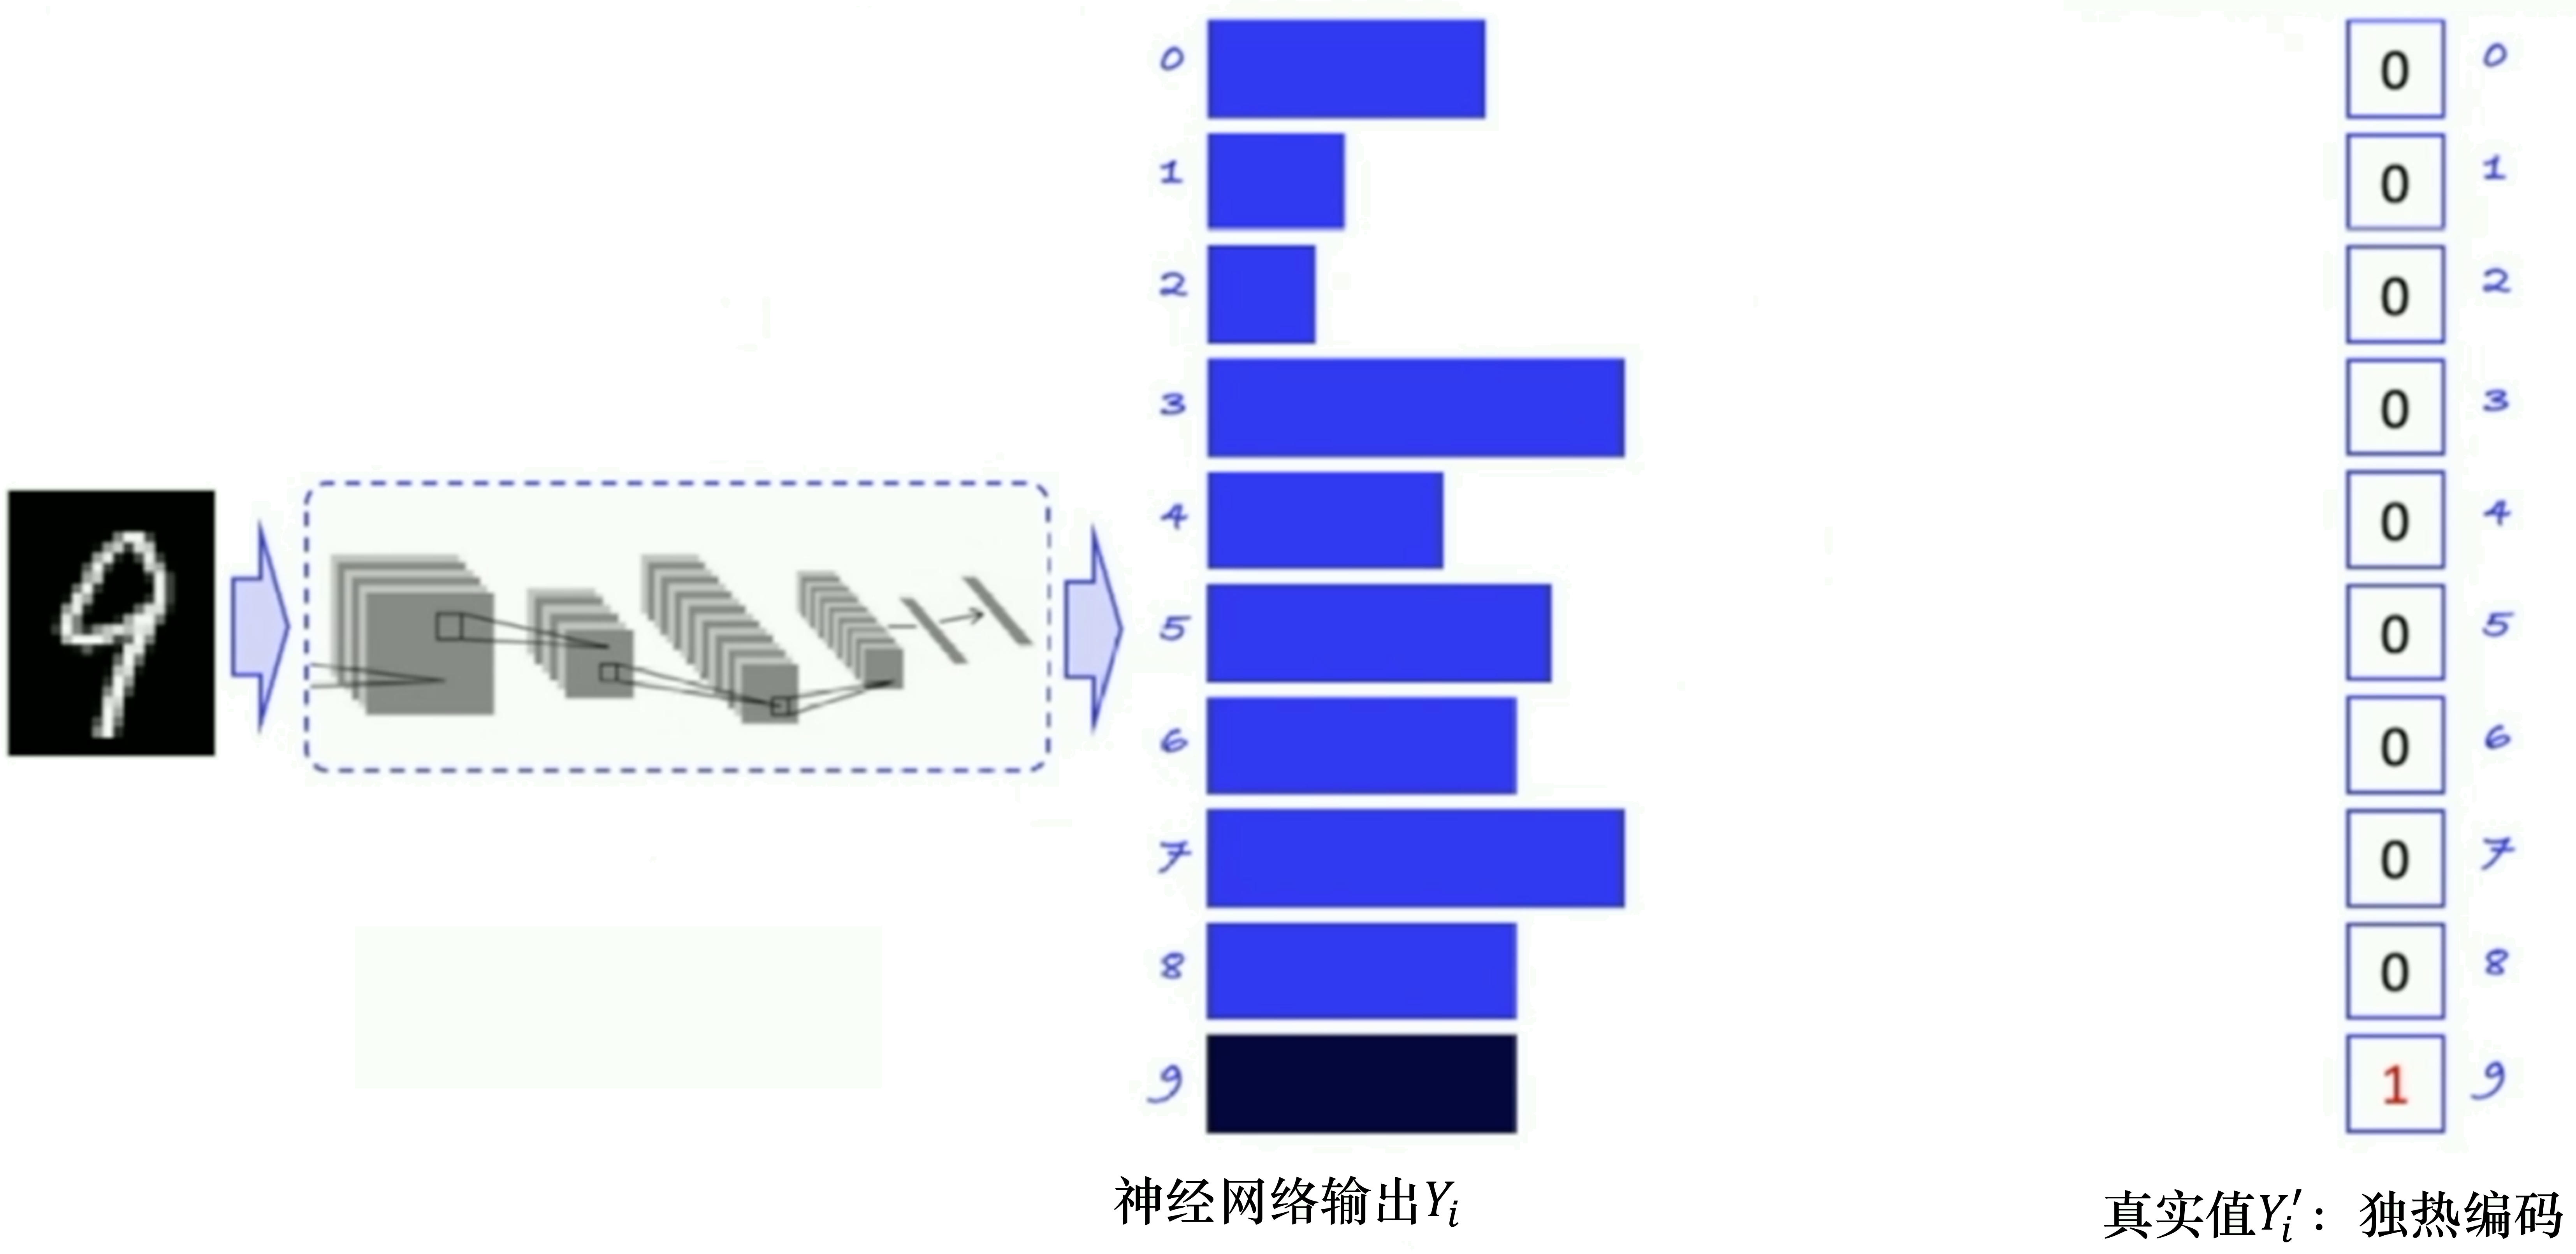
\includegraphics[width=0.5\linewidth]{ch6/figs/mnist_recognition.png}
    \caption{监督学习例子:手写数字识别}
    \label{fig:mnist_recognition}
\end{figure}

如\figref{fig:improve_nine_prob} 所示,我们所要做的就是提高输出 9 的概率,降低输出其他数字的概率,让神经网络输出的概率分布能够更贴近真实值的概率分布。我们可以用交叉熵来表示两个概率分布之间的差距。

\begin{figure}[hbt]
    \centering
    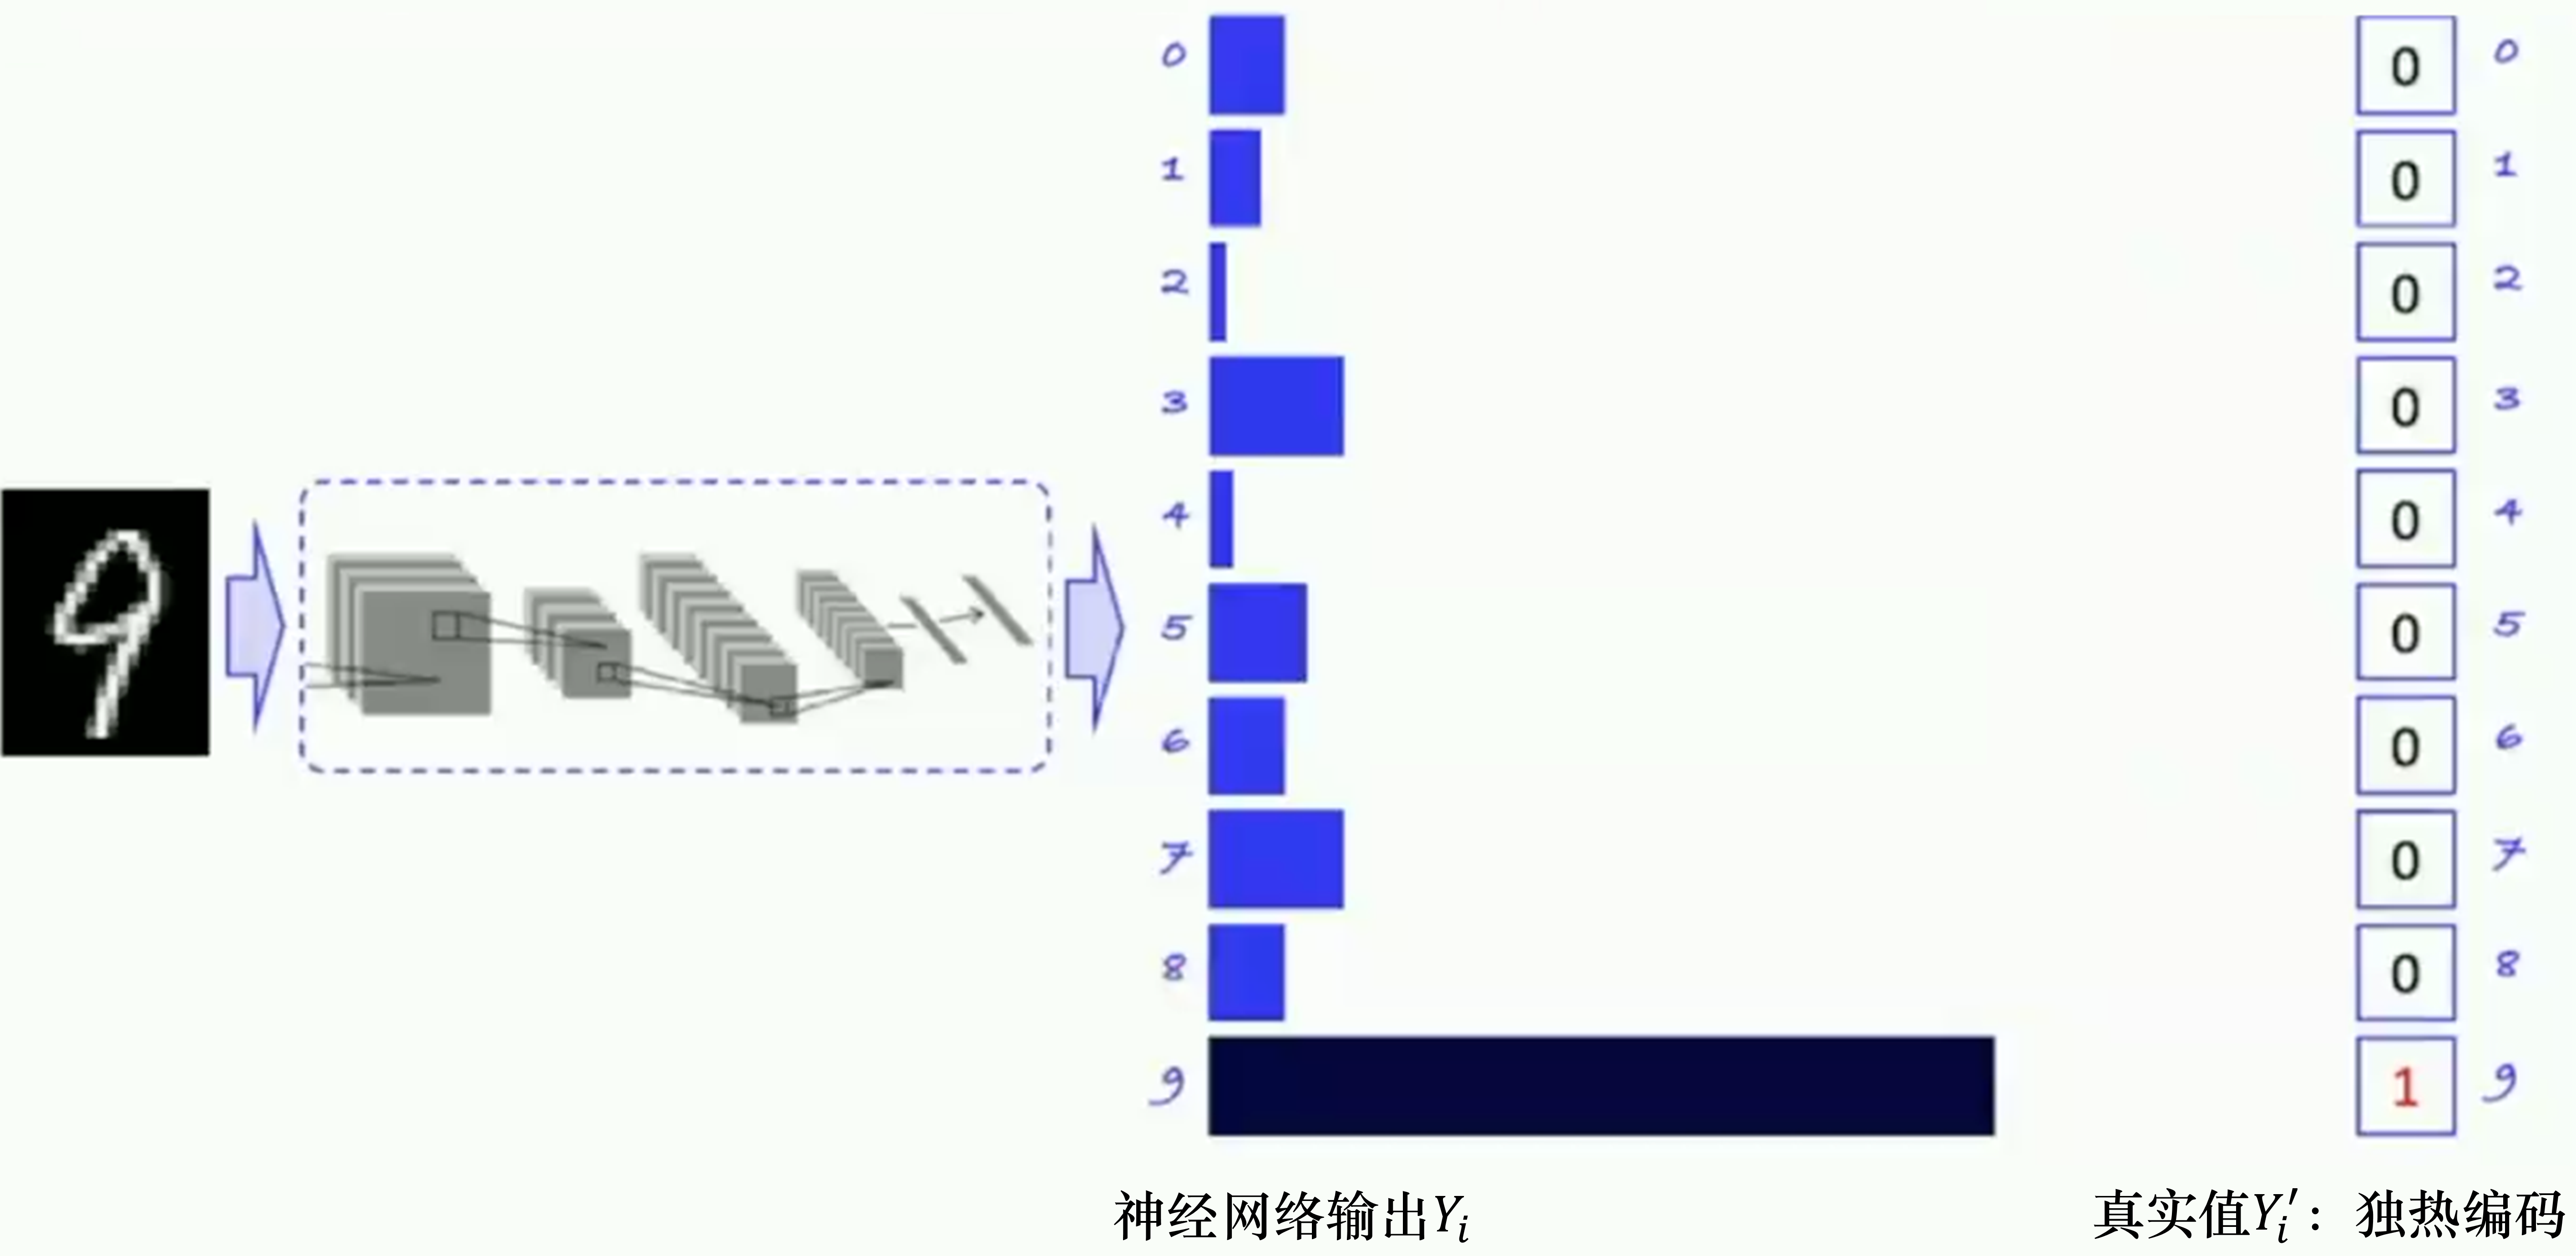
\includegraphics[width=0.5\linewidth]{ch6/figs/improve_nine_prob.png}
    \caption{提高数字9的概率}
    \label{fig:improve_nine_prob}
\end{figure}

我们看一下监督学习的优化流程,即怎么让输出逼近真实值。
如\figref{fig:opti_process} 所示,
监督学习的优化流程就是将图片作为输入传给神经网络,神经网络会判断图片中的数字属于哪一类数字,输出所有数字可能的概率,再计算交叉熵,即神经网络的输出 $Y_i$ 和真实的标签值 $Y_i'$ 之间的距离 $-\sum Y_{i}^{\prime} \cdot \log \left(Y_{i}\right)$。我们希望尽可能地缩小这两个概率分布之间的差距,计算出的交叉熵可以作为损失函数传给神经网络里面的优化器进行优化,以自动进行神经网络的参数更新。
\begin{figure}[hbt]
    \centering
    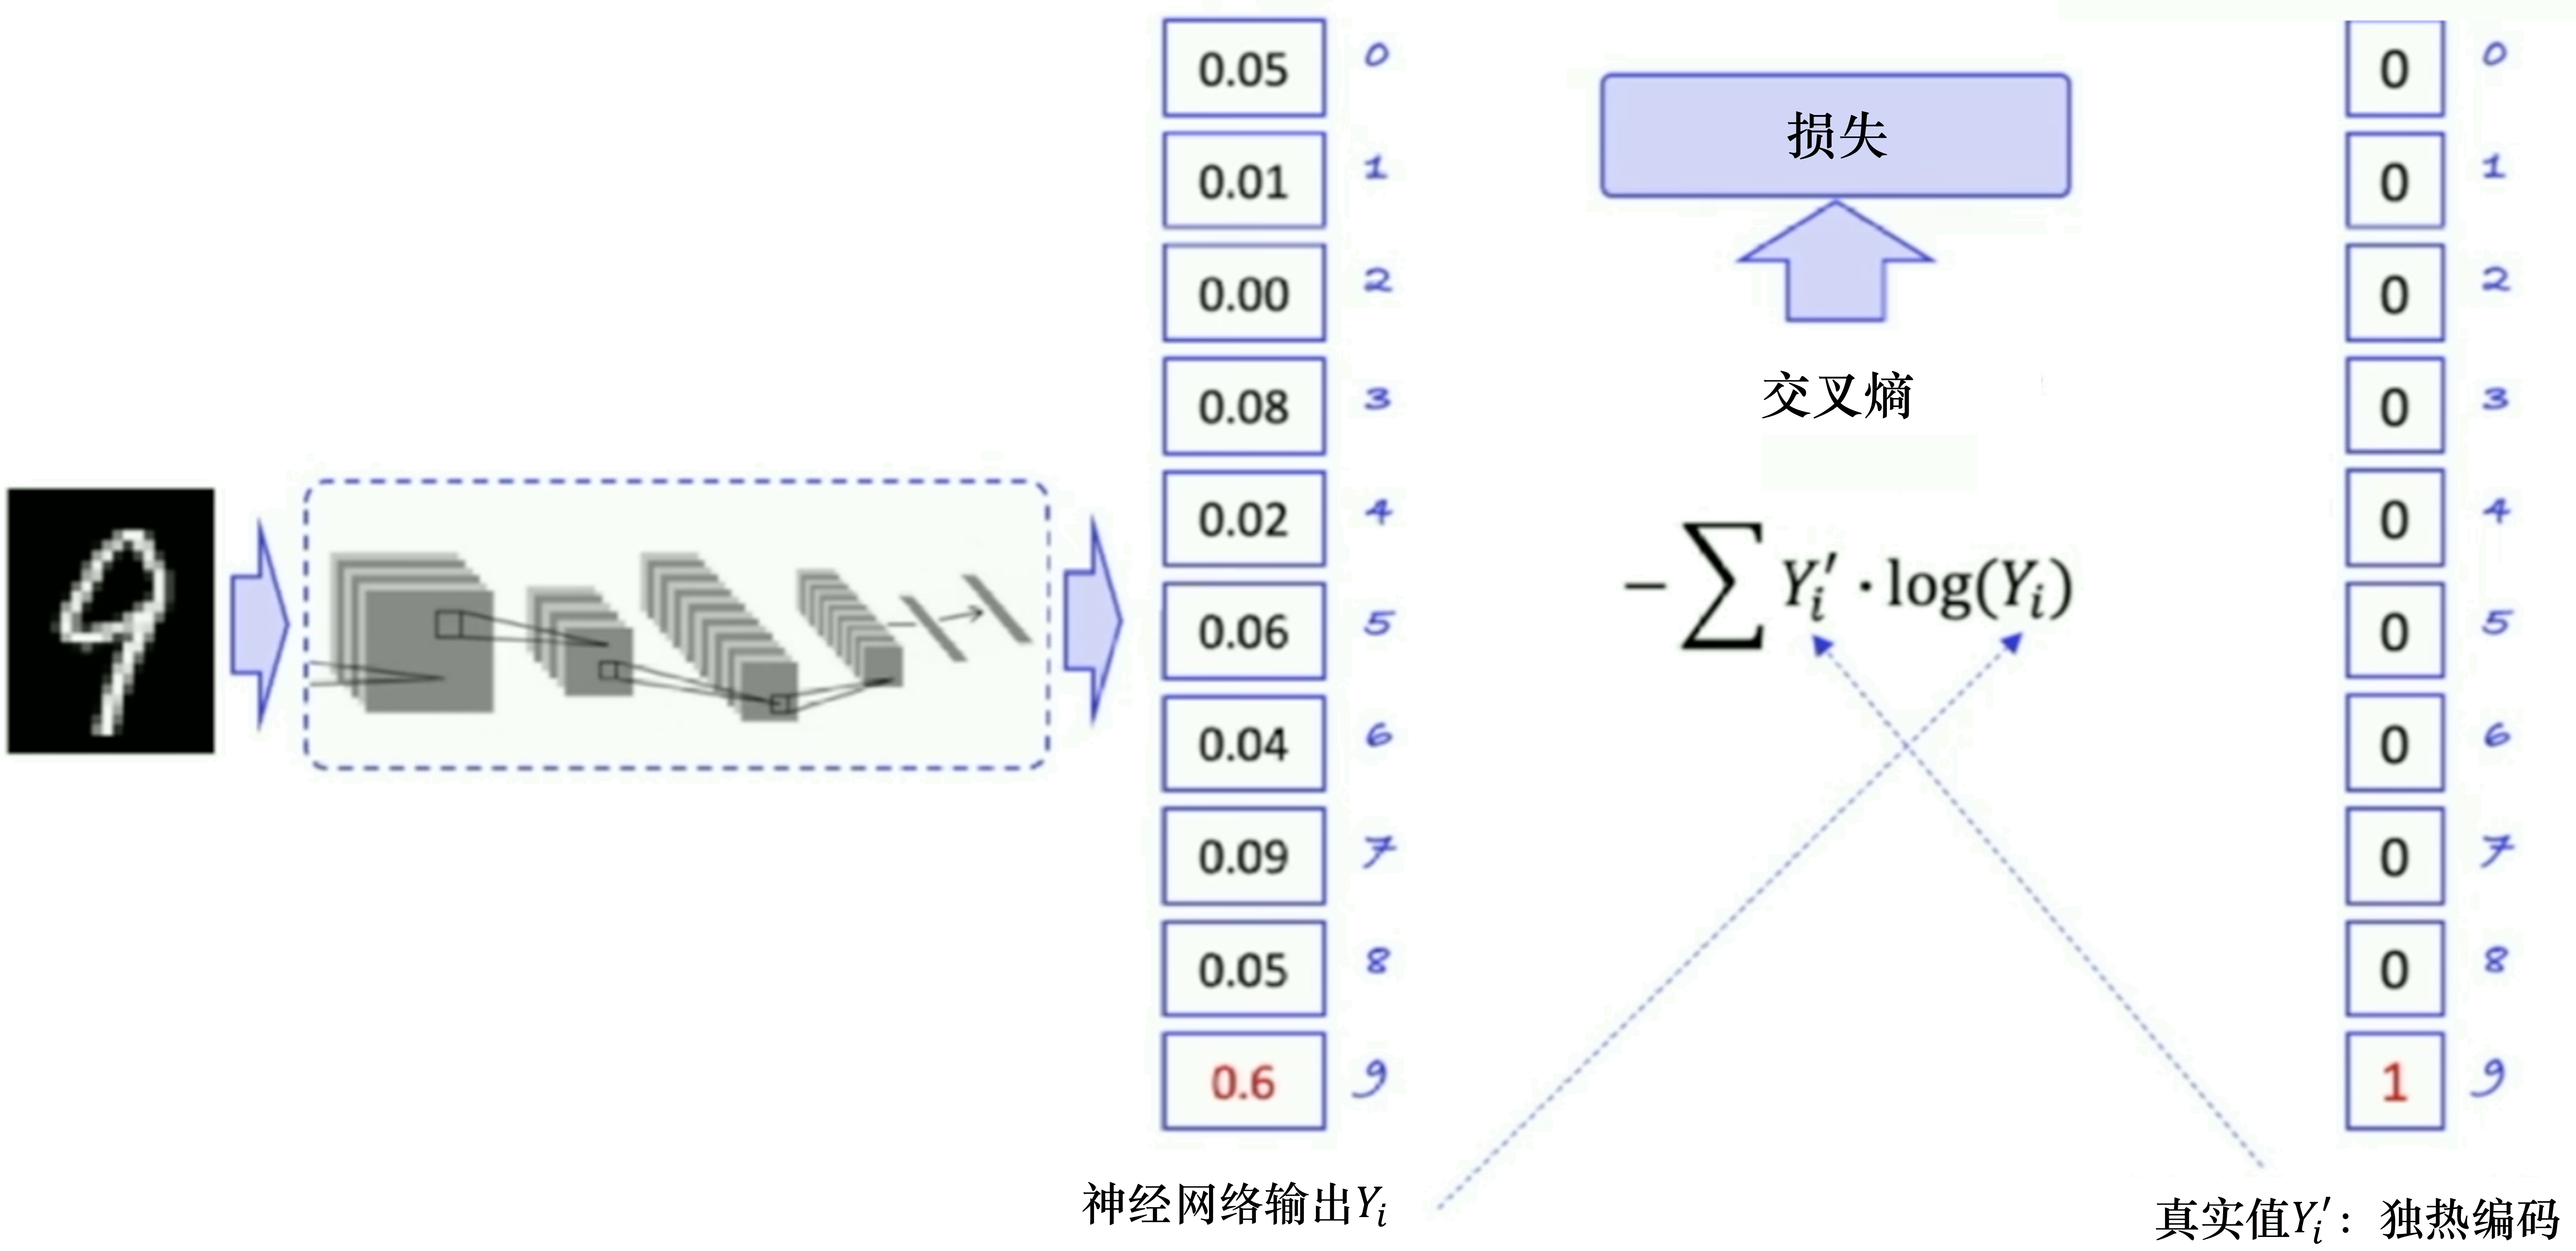
\includegraphics[width=0.5\linewidth]{ch6/figs/opti_process.png}
    \caption{优化流程}
    \label{fig:opti_process}
\end{figure}

类似地,如\figref{fig:pg_loss} 所示,策略梯度预测每一个状态下应该要输出的动作的概率,即输入状态 $s_t$,输出动作$a_t$的概率,比如 0.02、0.08、0.9。实际上输出给环境的动作是随机选择一个动作,比如我们选择向右这个动作,它的独热向量就是(0,0,1)。
我们把神经网络的输出和实际动作代入交叉熵的公式就可以求出输出动作的概率和实际动作的概率之间的差距。
但实际的动作 $a_t$ 只是我们输出的真实的动作,它不一定是正确的动作,它不能像手写数字识别一样作为一个正确的标签来指导神经网络朝着正确的方向更新,所以我们需要乘一个奖励回报 $G_t$。$G_t$相当于对真实动作的评价。
如果 $G_t$ 越大,未来总奖励越大,那就说明当前输出的真实的动作就越好,损失就越需要重视。
如果 $G_t$ 越小,那就说明动作 $a_t$ 不是很好,损失的权重就要小一点儿,优化力度也要小一点儿。
通过与手写数字识别的一个对比,我们就知道为什么策略梯度损失会构造成这样。
\begin{figure}[hbt]
    \centering
    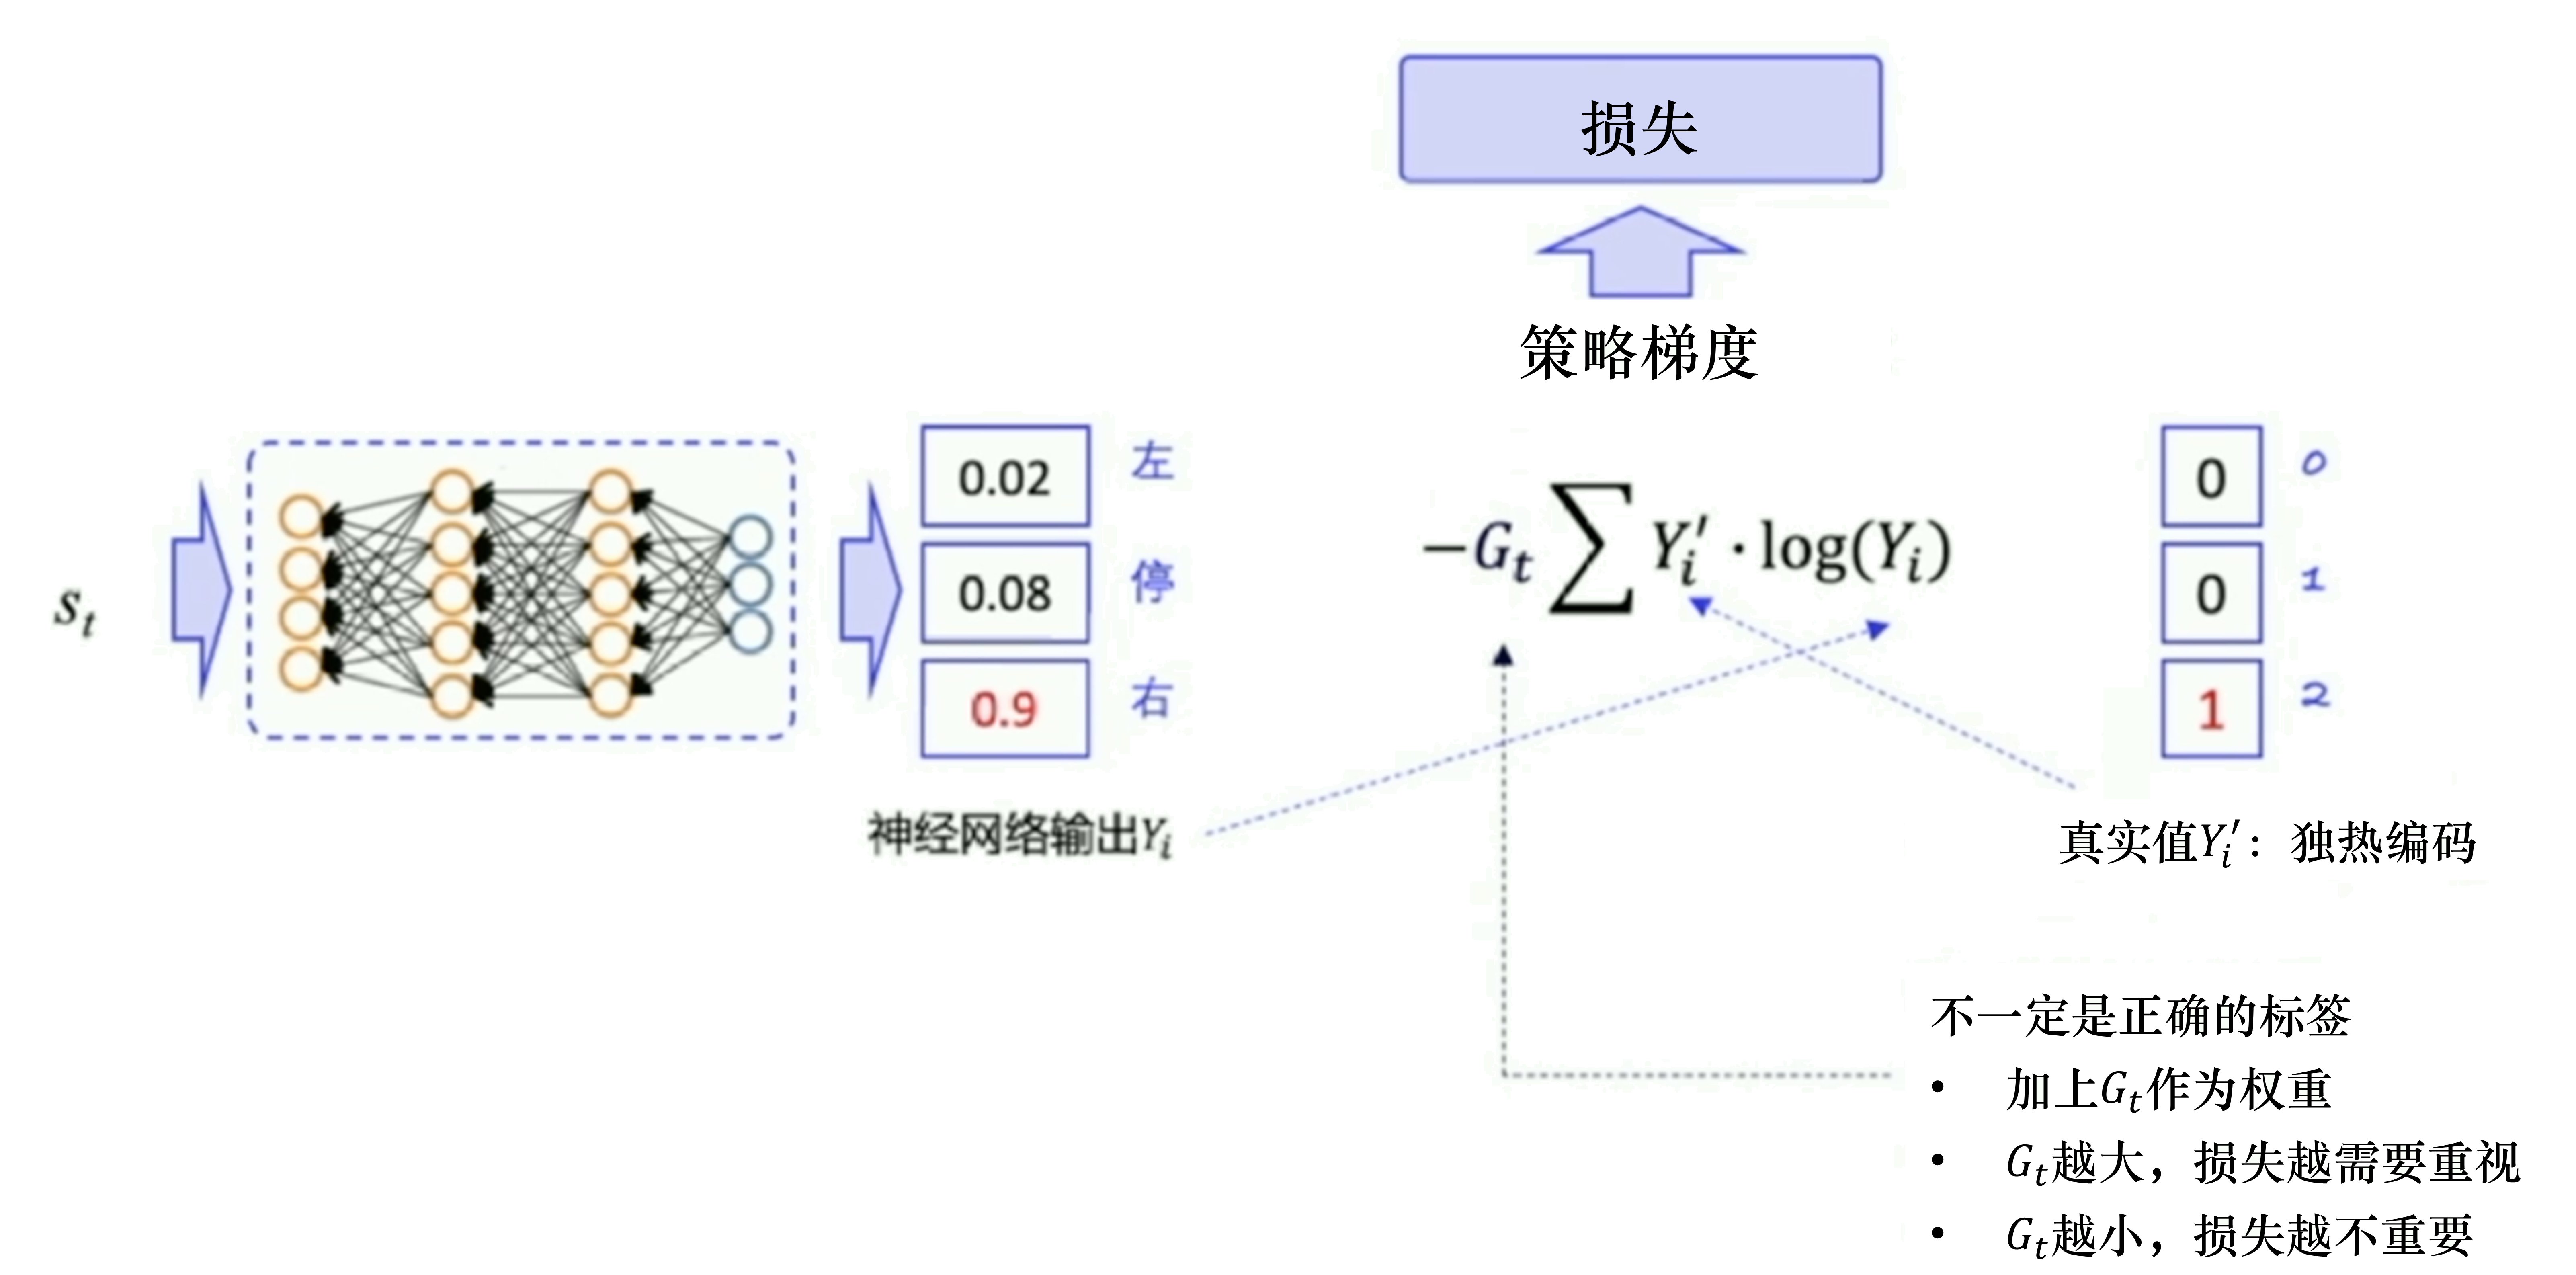
\includegraphics[width=0.5\linewidth]{ch6/figs/pg_loss.png}
    \caption{策略梯度损失}
    \label{fig:pg_loss}
\end{figure}

如\figref{fig:loss_compute} 所示,
实际上我们在计算策略梯度损失的时候,要先对实际执行的动作取独热向量,
% 拿到那个 $\ln \pi(a_t|s_t,\theta)$。我就拿实际执行的这个动作,
再获取神经网络预测的动作概率,将它们相乘,我们就可以得到 $\ln \pi(a_t|s_t,\theta)$,这就是我们要构造的损失。
因为我们可以获取整个回合的所有的轨迹,所以我们可以对这一条轨迹里面的每个动作都去计算一个损失。把所有的损失加起来,我们再将其“扔”给 Adam 的优化器去自动更新参数就好了。
\begin{figure}[hbt]
    \centering
    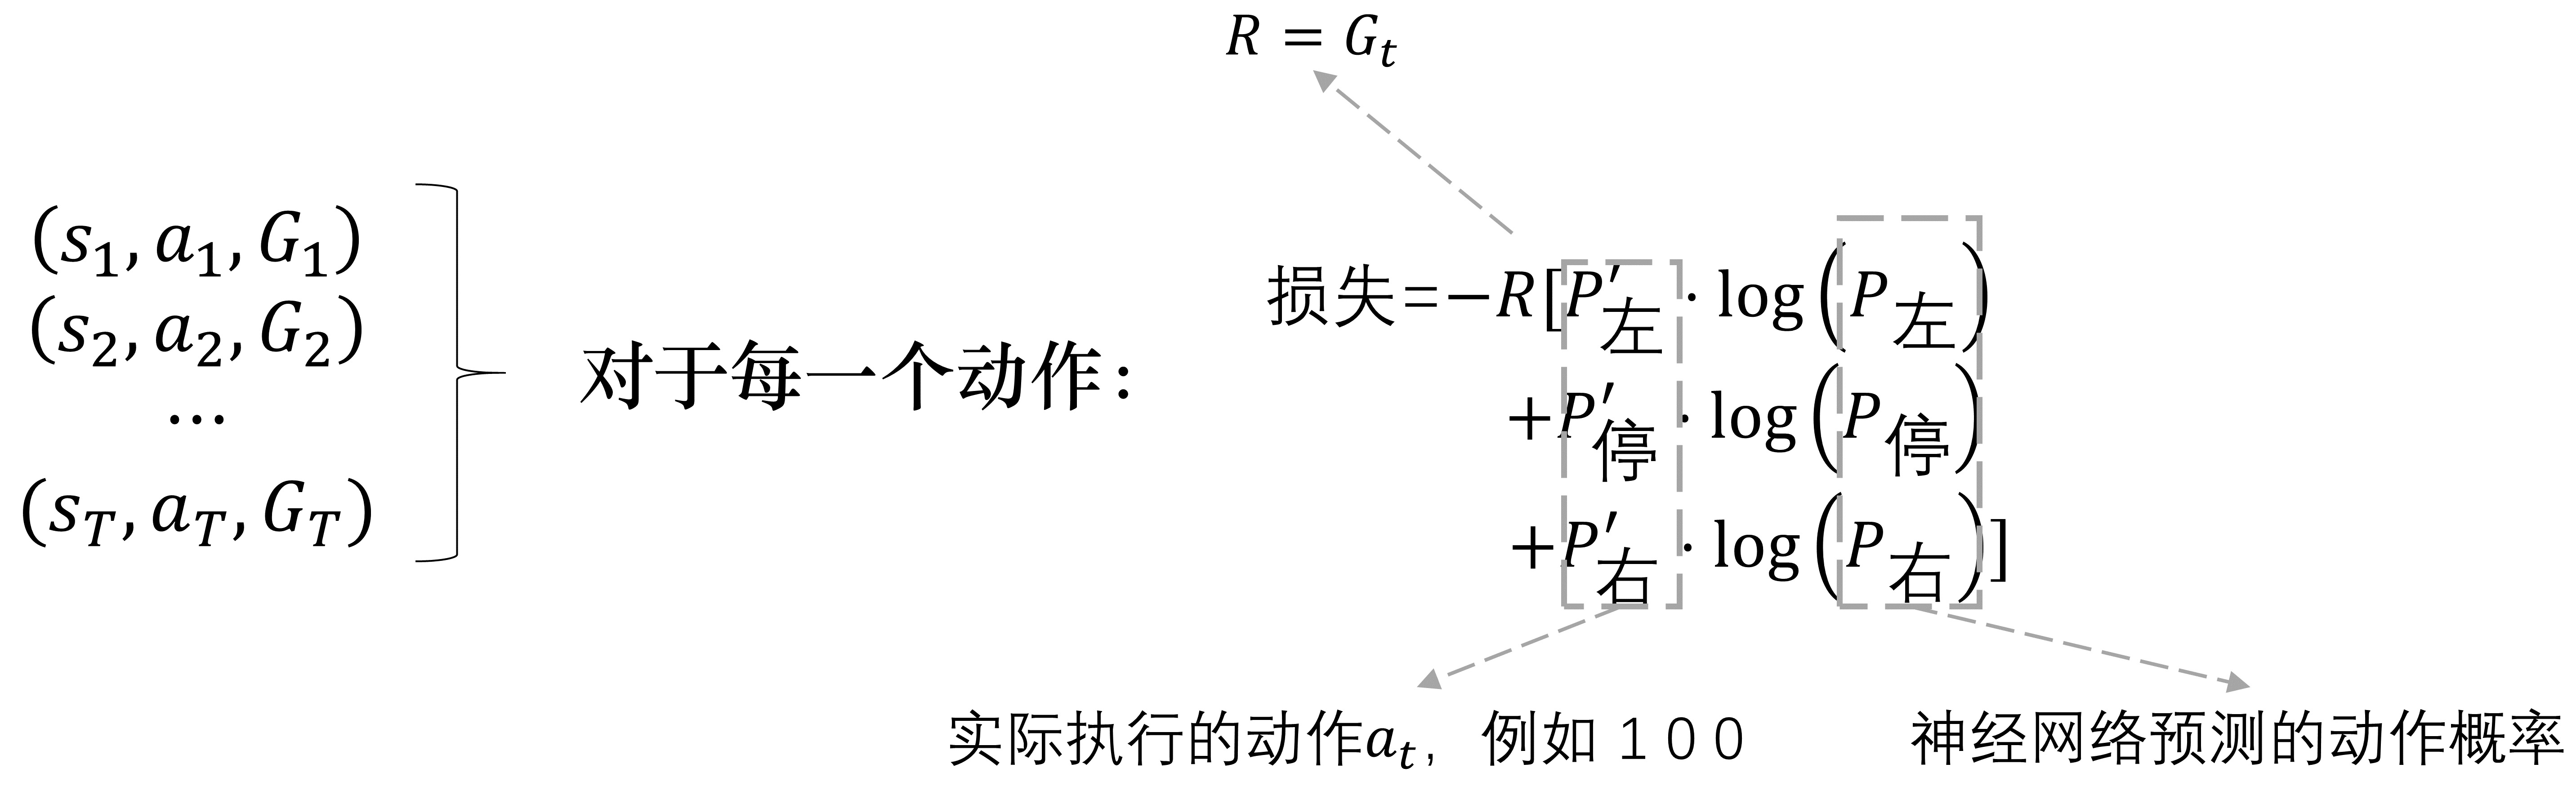
\includegraphics[width=0.5\linewidth]{ch6/figs/loss_compute.png}
    \caption{损失计算}
    \label{fig:loss_compute}
\end{figure}

\figref{fig:REINFORCE_process} 所示为 REINFORCE 算法示意图,首先我们需要一个策略模型来输出动作概率,输出动作概率后,
通过 \kw{sample()} 函数得到一个具体的动作,与环境交互后,我们可以得到整个回合的数据。得到回合数据之后,我们再去执行\kw{learn()} 函数,在 \kw{learn()} 函数里面,我们就可以用这些数据去构造损失函数,“扔”给优化器优化,更新我们的策略模型。
\begin{figure}[hbt]
    \centering
    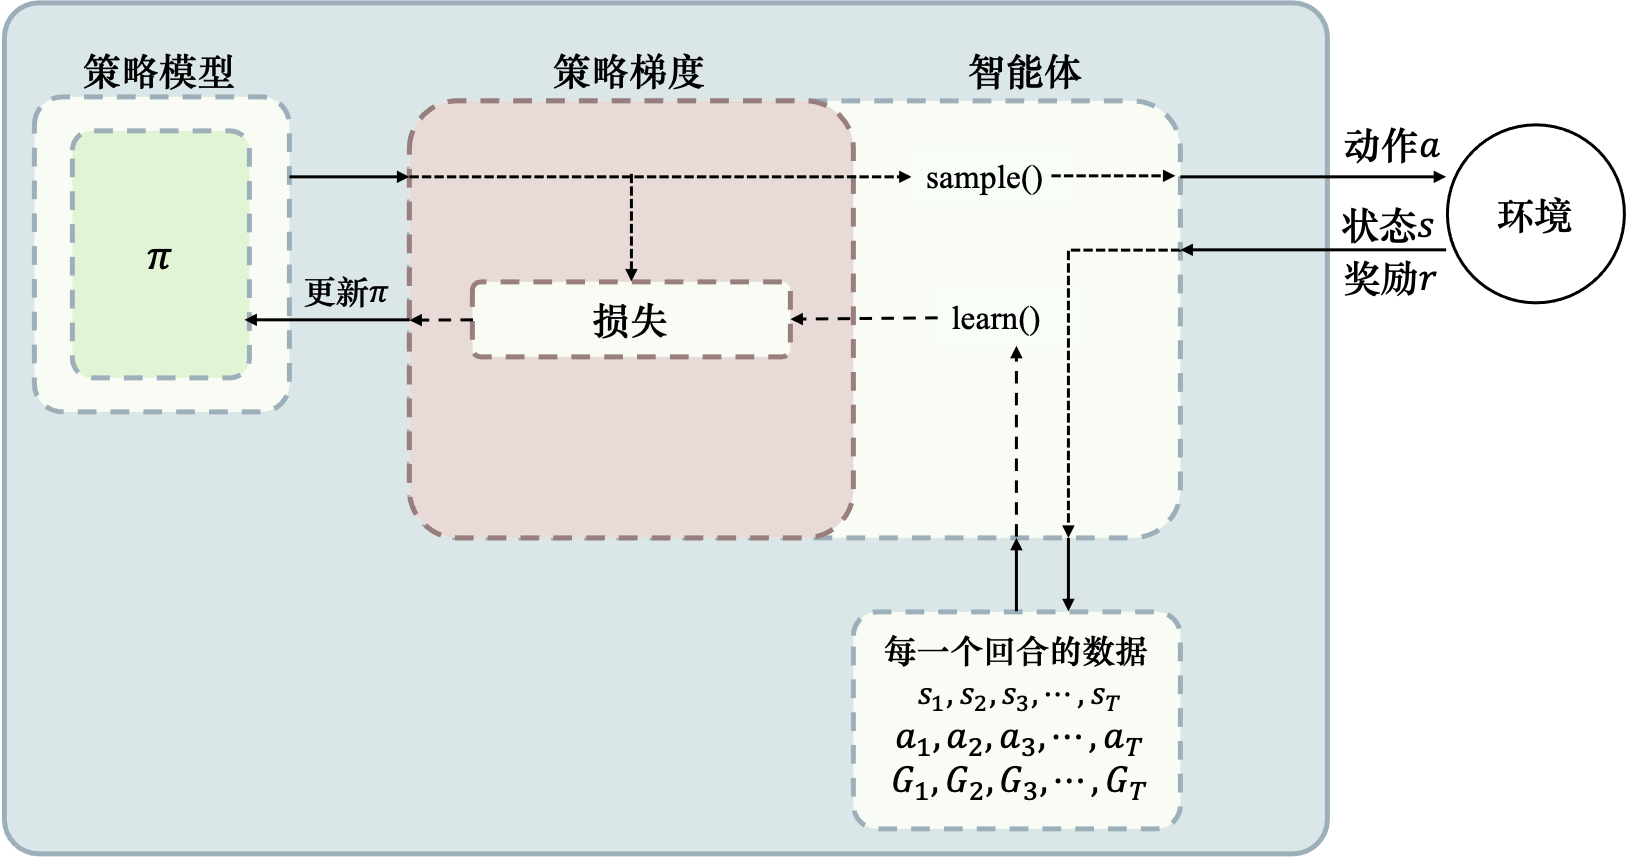
\includegraphics[width=0.5\linewidth]{ch6/figs/REINFORCE_process.png}
    \caption{REINFORCE算法示意}
    \label{fig:REINFORCE_process}
\end{figure}

\subsection{策略梯度的进阶推导}

在上一节中我们通过计算轨迹的概率并乘上对应的价值,然后将通过全期望公式将这些项累加起来就得到了关于策略的总价值期望,即我们要求得的目标函数,如\eqref{eq:expect_policy_2}所示。
\begin{equation}
    \label{eq:expect_policy_2}
    \begin{aligned}
    J(\pi_{\theta}) = P_{\theta}(\tau_{1})R(\tau_{1})+P_{\theta}(\tau_{2})R(\tau_{2})+\cdots \\
    &=\int_\tau P_{\theta}(\tau) R(\tau) \\ 
\end{aligned}
\end{equation}
然后通过对数微分等技巧求出对应的梯度,如\eqref{eq:pg_ob_grad_2}所示。
\begin{equation}
    \label{eq:pg_ob_grad_2}
    \begin{aligned}
    \nabla_\theta J\left(\pi_\theta\right) = \underset{\tau \sim \pi_\theta}{\mathrm{E}}\left[\sum_{t=0}^T \nabla_\theta \log \pi_\theta\left(a_t \mid s_t\right) R(\tau)\right]
    \end{aligned}
\end{equation}

那么问题来了,可以看到无论是目标函数还是对应的梯度都必须求出关于轨迹$\tau$的项,例如$R(\tau)$。乍一看这个包含轨迹的项似乎比较容易求,但实际上是很难的,就像我们某些玩家日常指挥别人打游戏时那样,嘴上说说容易,实际操作起来却发现处处是细节。为什么说处处是细节呢?注意看\eqref{eq:pg_ob_grad_2}中对于$\log \pi_\theta\left(a_t \mid s_t\right)$中的每一个状态-动作对$(s_t,a_t)$,我们都需要求出对应的累积奖励$R(\tau)$。我们当然可以先把每一条从初始状态$s_0$到当前状态$s_t$所经历的轨迹对应的每一步奖励存储起来然后求出最终的累积奖励$R(\tau)$,即便 REINFORCE 算法在计算轨迹对应的价值方面做了一定的优化,但一个状态$s_t$背后的累积价值和梯度是需要通过包含很多个历史状态的轨迹来计算的,光是这样想恐怕读者们眼泪都要止不住掉下来。其次我们观察\eqref{eq:expect_policy_2},我们是要将所有轨迹的概率和对应的累积奖励相乘然后累加得到最终的价值期望,也就是目标函数。那么这里所有的轨迹是哪些轨迹呢?怎么数出来的?可能有些读者会说我们可以先搜集一些轨迹来近似所有轨迹,那么到底要搜集多少条轨迹才能近似?当然你可以搜集成千上万条,但恐怕还没等你计算完这些轨迹的期望其他人可能都已经用 DQN 算法完美解决这个问题了。我们原本认为直接通过对策略的梯度进行优化会比以间接的方式先估计对应的价值然后选择动作收敛的速度要更快,如果计算轨迹期望都这么麻烦似乎失去了实现策略梯度算法的初衷。并且还有一个很重要的问题,如\figref{fig:traj_compute}所示(补一张类似于条条大路通罗马的可爱动漫图),实际过程中初始状态$s_0$到当前状态$s_t$的轨迹应该不止一条,我可能走一步就到了状态$s_t$,也可能走了很多步才到$s_t$,走一步和走很多步生成的轨迹对应的累积奖励多数情况下也是不一样的,这个时候我们是多个轨迹都算进去还是只考虑其中一条呢?

\begin{figure}[hbt]
    \centering
    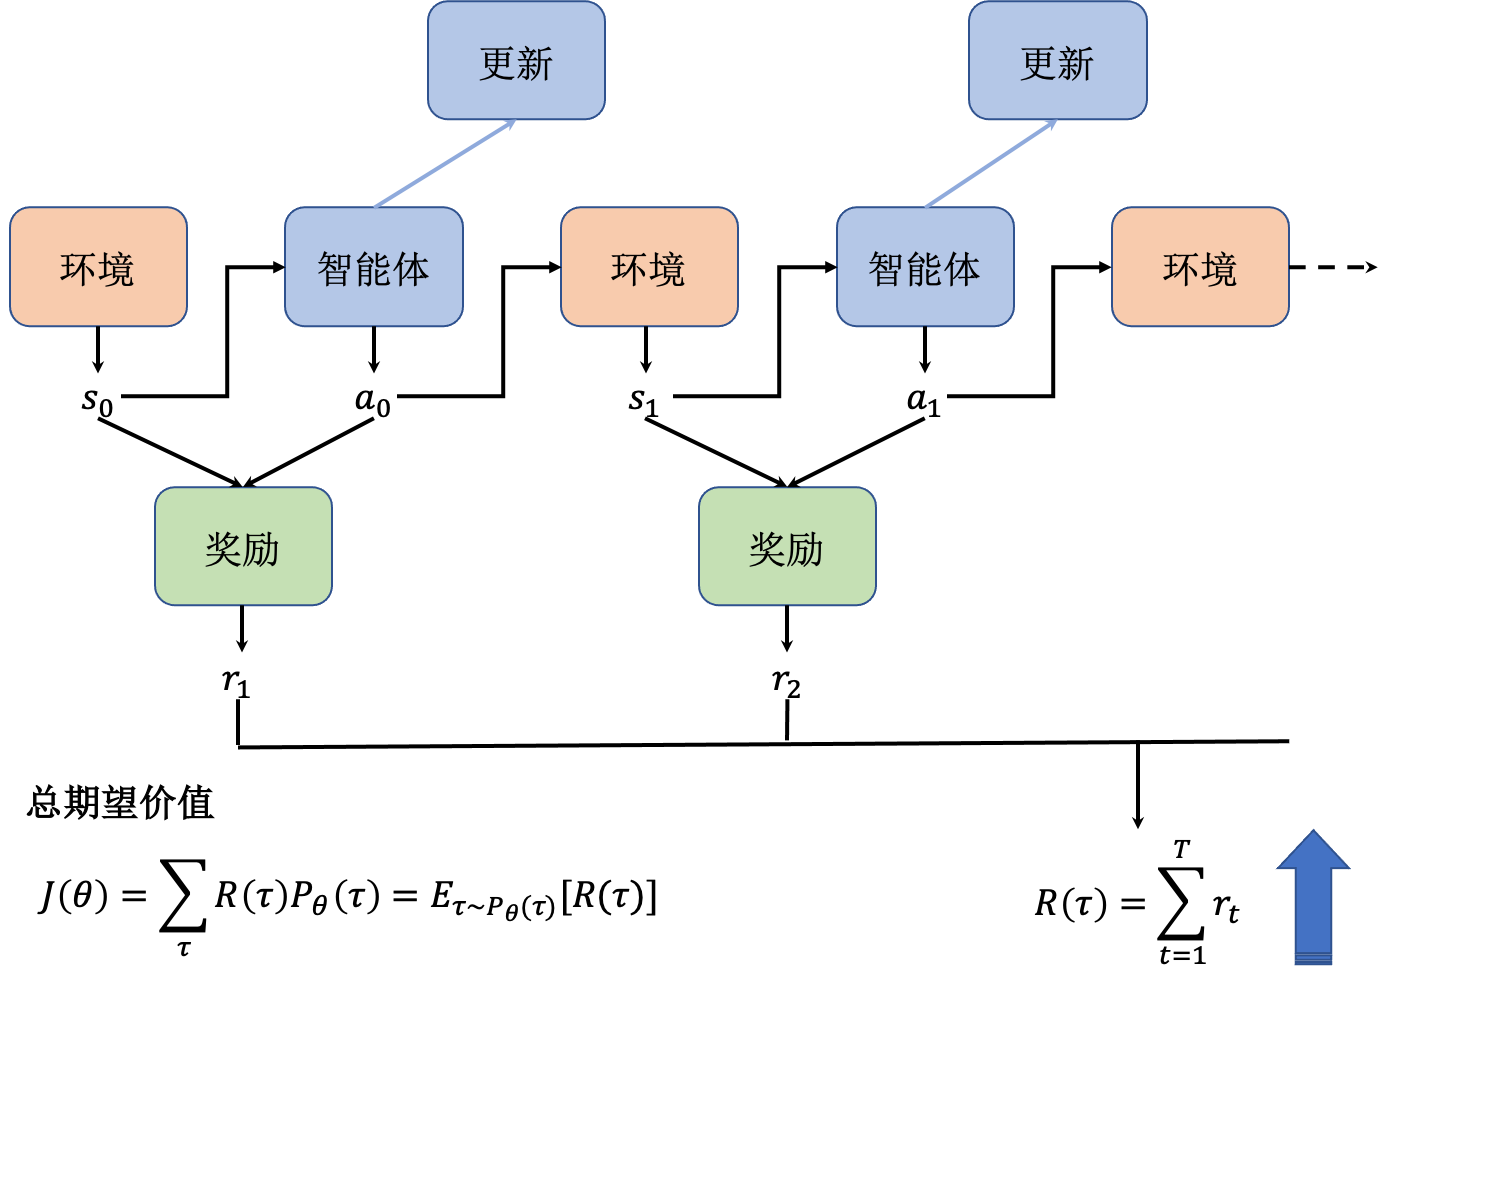
\includegraphics[width=0.5\linewidth]{ch6/figs/expected_reward.png}
    \caption{轨迹的计算}
    \label{fig:traj_compute}
\end{figure}

这样绕来绕去始终得不到一个准确的答案,这个时候可能就会有读者灵光乍现,我们在马尔科夫决策过程中计算的奖励不应该是“长期奖励”吗?那么这时候恭喜你没有被调皮的作者绕进去!实际上,在所有的马尔可夫过程中我们优化的目标都是“长期”的价值期望,不明白的读者可以再温习一下马尔可夫决策过程的定义以及前面Q learning算法相关的推导内容,相信你一定能够回顾起来所谓“长期”的意义。暂时给一个小的结论,我们这里选择的轨迹和对应的累积价值都应该是长期的轨迹和价值,如此才能保证我们的目标函数计算出来的也是长期的总价值。换句话说,对于每条轨迹,从初始状态$s_0$到当前状态$s_t$所经历的步数应该是无限的,即$t \rightarrow \infty$。这时候读者可能会奇怪,有限步数就已经够难算了,无限步数还能算出来吗?答案是可以的,而且更简便快捷,在数学中就是这样,“无限的”往往比“有限的”更容易计算出来,这里就涉及到一个重要的概念,即马尔可夫链的平稳分布,还请跟随笔者的思路到下一小节详细了解什么是马尔可夫链的平稳分布。

\subsubsection{平稳分布}

在本小节中我们将会详细了解什么是马尔可夫链的平稳分布,先不急着抛出一堆抽象的概念和公式,我们先来看一个经典的例子。这个例子是这样的,社会学家在他们的研究中通常会把人按照经济状况分成三类:上层,中层和下层,这三层就代表着三种状态,我们分别用 1,2,3 来表示。并且社会学家还发现决定一个人经济阶层的最重要因素就是其父母的收入阶层,即如果一个人的经济阶层为上层,那么他的孩子会有 0.5 的概率继续处于上层,也会有 0.4 的概率变成中层,更有 0.1 的概率降到下层,当然这些概率数值只是笔者拍脑袋想出来以便于后面的计算的,并没有一定的统计依据。这些概率其实就是我们所说的马尔可夫链中的转移概率,同样对于其他经济阶层的人他们的孩子也会有一定的概率变成上、中、下的任一经济阶层,如\figref{fig:markov_economy}所示。

\begin{figure}[hbt]
    \centering
    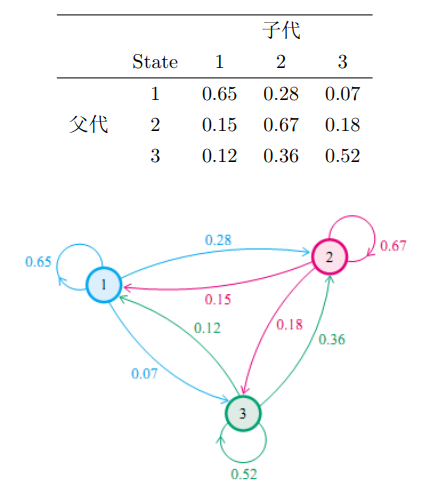
\includegraphics[width=0.5\linewidth]{ch6/figs/markov_economy.png}
    \caption{期望的奖励}
    \label{fig:markov_economy}
\end{figure}

这样我们就可以列出转移概率矩阵,如\eqref{eq:tran_prob_economy}所示。

\begin{equation}
    \label{eq:tran_prob_economy}
    P=\left[\begin{array}{lll}
    0.5 & 0.4 & 0.1 \\
    0.2 & 0.6 & 0.2 \\
    0.05 & 0.45 & 0.5
    \end{array}\right]
\end{equation}

我们假设有这么一批数量足够的人,称之为第 1 代人,他们的经济阶层比例为$\pi_0=[0.15,0.62,0.23]$,那么根据上面的转移概率矩阵我们就可以求出第二代的阶层比例。怎么求呢?首先求出第二代上层的比例,我们知道第一代人中有 0.15 的比例是上层,这 0.15 比例的人中子代为上层的概率是 0.5, 而第一代人中 0.62 比例的中层会有 0.2 的概率流入上层,0.23 比例的下层中其子代也会有 0.05 的概率流入上层,那么最后第二代上层的比例就为 $0.15 \times 0.5 + 0.62 \times 0.2 + 0.23 \times 0.05 = 0.2105 \approx 0.210$,依次类推,第二代中层的比例为$0.15 \times 0.4 + 0.62 \times 0.6 + 0.23 \times 0.45 \approx 0.536$,第二代下层的比例为$0.254$,这样我们就能得出第二代的阶层比例为$\pi_1=[0.210,0.536,0.254]$。这里细心的读者会发现不需要这么麻烦的计算过程,只要学过线性代数利用矩阵向量相乘就能得到,即$\pi_1 = \pi_0 P = [0.210,0.536,0.254]$。同理,第二代人的比例也可以求出,即 $\pi_2 = \pi_1 P = \pi_0 P^2$,依次类推,第n代人的比例为$\pi_n = \pi_0 P^n$。既然这本书同时也是教大家如何代码实战的,这里我们 Python 代码来求出前 10 代人的比例,如下。


\begin{lstlisting}[language=Python]
import numpy as np
pi_0 = np.array([[0.15,0.62,0.23]])
P = np.array([[0.5,0.4,0.1],[0.2,0.6,0.2],[0.05,0.45,0.5]])
for i in range(1,10+1):
    pi_0 = pi_0.dot(P)
    print(f"第{i}代人的比例为:")
    print(np.around(pi_0,3))
\end{lstlisting}

我们可以很快获得计算的结果,如下。

\begin{lstlisting}[language=Bash]
第1代人的比例为:
[[0.211 0.536 0.254]]
第2代人的比例为:
[[0.225 0.52  0.255]]
第3代人的比例为:
[[0.229 0.517 0.254]]
第4代人的比例为:
[[0.231 0.516 0.253]]
第5代人的比例为:
[[0.231 0.516 0.253]]
第6代人的比例为:
[[0.231 0.516 0.253]]
第7代人的比例为:
[[0.232 0.516 0.253]]
第8代人的比例为:
[[0.232 0.516 0.253]]
第9代人的比例为:
[[0.232 0.516 0.253]]
第10代人的比例为:
[[0.232 0.516 0.253]]
\end{lstlisting}

这里忽略程序算出来的小数取舍问题,比如第一代人我们手算的比例而$[0.210,0.536,0.254]$,而程序却是$[0.211,0.536,0.254]$,这是因为程序内置保留有效数字的规则问题,不影响整体结果。回归正题,从上面的结果中,我们发现从第5代开始经济阶层的比例开始神奇地固定了下来。换句话说,无论初始状态是什么,经过多次概率转移之后都会存在一个稳定的状态分布。其次我们只需要知道这个稳定的分布并乘以对应的价值,就可以计算所谓的长期收益了。

现在我们可以正式地总结一下马尔可夫链的平稳分布了,对于任意马尔可夫链,如果满足以下两个条件:

\begin{itemize}
    \item 非周期性:由于马尔可夫链需要收敛,那么就一定不能是周期性的,实际上我们处理的问题基本上都是非周期性的,这点不需要做过多的考虑。
    \item 状态连通性:即存在概率转移矩阵$P$,能够使得任意状态$s_0$经过有限次转移到达状态$s$,反之亦然。
\end{itemize}

这样我们就可以得出结论,即该马氏链一定存在一个平稳分布,我们用$d^{\pi}(s)$表示,可得到\eqref{eq:markov_station}:

\begin{equation}
    \label{eq:markov_station}
    d^\pi(s)=\lim _{t \rightarrow \infty} P\left(s_t=s \mid s_0, \pi_\theta\right)
\end{equation}

我们回顾前面小节中计算轨迹概率的公式$P_{\theta}(\tau)$,可以发现如果轨迹$\tau$的初始状态是$s_0$并且终止状态是$s$的话,轨迹概率公式$P_{\theta}(\tau)$跟平稳分布的$d^\pi(s)$是等效的,当然前提是该条轨迹必须“无限长”,即$t \rightarrow \infty$。但是平稳分布与轨迹概率公式相比,它的好处就是只涉及一个定量即初始状态$s_0$和一个变量$s$。对于每个状态$s$,我们用$V^{\pi}(s)$表示策略$\pi$下对应的价值,读者们现在可以往前回顾,为什么笔者说策略梯度算法跟基于价值函数的算法都是在计算累积状态的价值期望了,此时策略梯度算法目标函数就可以表示为\eqref{eq:pg_station_object}。

\begin{equation}
    \label{eq:pg_station_object}
    J(\theta)=\sum_{s \in \mathcal{S}} d^\pi(s) V^\pi(s)=\sum_{s \in \mathcal{S}} d^\pi(s) \sum_{a \in \mathcal{A}} \pi_\theta(a \mid s) Q^\pi(s, a)
\end{equation}

同样可以利用对数微分技巧求得对应的梯度,如\eqref{eq:pg_station_object_grad}。

\begin{equation}
    \label{eq:pg_station_object_grad}
    \begin{aligned}
    \nabla_\theta J(\theta) & \propto \sum_{s \in \mathcal{S}} d^\pi(s) \sum_{a \in \mathcal{A}} Q^\pi(s, a) \nabla_\theta \pi_\theta(a \mid s) \\
    &=\sum_{s \in \mathcal{S}} d^\pi(s) \sum_{a \in \mathcal{A}} \pi_\theta(a \mid s) Q^\pi(s, a) \frac{\nabla_\theta \pi_\theta(a \mid s)}{\pi_\theta(a \mid s)} \\
    &=\mathbb{E}_\pi\left[Q^\pi(s, a) \nabla_\theta \log \pi_\theta(a \mid s)\right]
    \end{aligned}
\end{equation}

可以发现该梯度跟前面小节求出的\eqref{eq:pg_ob_grad_2}的形式是类似的,只是变量从轨迹$\tau$换成了状态$s$,更便于实际问题的求解。在本书前面所讲的值迭代算法中,我们优化的目标是所有状态对应的$V(s)$,值迭代算法解决的问题是马尔可夫奖励过程。而强化学习的基本问题是马氏决策过程,因此在 Q learning 或 DQN 算法中,我们优化的是所有状态对应的 Q 值$Q^\pi(s, a)$,其中$Q^\pi(s, a)=\sum_{a \in \mathcal{A}} \pi(a \mid s) Q^\pi(s, a)$,优化所有的 Q 值之后再使用$\varepsilon - greedy$之类的策略选择动作。而在策略梯度算法中,我们是同时优化策略部分$\nabla_\theta \log \pi_\theta(a \mid s)$和价值部分$Q^\pi(s, a)$的,其中策略部分我们一般叫做 Actor ,价值部分叫做 Critic 。到这里就已经不是简单的纯策略梯度算法了,而是同时结合了基于价值和策略梯度的算法,我们一般把这类算法称之为 Actor-Critic 算法。这里 Actor 或者说策略梯度算法相比于基于价值的算法,其最大的好处就是同时可以适用于离散动作和连续动作空间的环境,而仅仅基于价值的算法比如 DQN 等算法只能适用于离散动作空间的问题。此外基于价值的算法只能通过众多动作价值中选择出一个最大价值对应的动作,是确定性的,而策略梯度算法中的 Actor 可以用一些随机分布比如高斯分布来表示,即能够使用随机策略。而有些实际问题的最优策略恰恰是随机策略,这种情况下基于价值的算法也无法解决。而这里的 Critic 使用了 DQN 算法中的 Q 值来表示,但是也会有更好的表示方法,这点我们将在后续讲解 A2C 和 GAE 等算法的章节中详细展开。我们将在下一小节中先简要介绍一下 Actor 的常用设计方式。

\subsubsection{策略函数的设计}

这一小节中我们将简要讲述 Actor 的常用设计方式,也就是策略函数$\pi_\theta(a \mid s)$。 对于离散动作空间的问题,最常用的策略函数就是 softmax 函数,softmax 函数在深度学习中通常作为最后一层网络用于多分类,而在强化学习中则使用描述状态和行为的特征函数$\phi(s,a)$和参数$\theta$的线性组合来权衡一个动作发生的概率,如\eqref{eq:softmax_act}:


\begin{equation}
    \label{eq:softmax_act}
    \pi_\theta(s, a)=\frac{e^{\phi(s, a)^T} \theta}{\sum_b e^{\phi(s, b)^T}}
\end{equation}

对应的梯度也可方便求得,如\eqref{eq:softmax_act_grad}。

\begin{equation}
    \label{eq:softmax_act_grad}
    \nabla_\theta \log \pi_\theta(s \mid a)=\phi(s, a)-\mathbb{E}_{\pi_\theta}[\phi(s, .)]
\end{equation}

而对于连续动作空间,通常策略对应的动作可以从高斯分布${\mathbb{N}}\left(\phi(s)^{\mathbb{T}} \theta, \sigma^2\right)$,对应的梯度也可求得:
\begin{equation}
    \nabla_\theta \log \pi_\theta(s, a)==\frac{\left(a-\phi(s)^T \theta\right) \phi(s)}{\sigma^2}
\end{equation}

\subsection{关键词}

策略(policy):在每一个演员中会有对应的策略,这个策略决定了演员的后续动作。具体来说,策略就是对于外界的输入,输出演员现在应该要执行的动作。一般地,我们将策略写成 $\pi$ 。

回报(return):一个回合(episode)或者试验(trial)得到的所有奖励的总和,也被人们称为总奖励(total reward)。一般地,我们用 $R$ 来表示它。

轨迹(trajectory):一个试验中我们将环境输出的状态 $s$ 与演员输出的动作 $a$ 全部组合起来形成的集合称为轨迹,即 $\tau=\left\{s_{1}, a_{1}, s_{2}, a_{2}, \cdots, s_{t}, a_{t}\right\}$ 。

奖励函数(reward function):用于反映在某一个状态采取某一个动作可以得到的奖励分数,这是一个函数。即给定一个状态-动作对 ($s_1$,$a_1$) ,奖励函数可以输出 $r_1$ 。给定 ($s_2$,$a_2$),它可以输出 $r_2$。 把所有的 $r$ 都加起来,我们就得到了 $R(\tau)$ ,它代表某一个轨迹 $\tau$ 的奖励。

期望奖励(expected reward):$\bar{R}_{\theta}=\sum_{\tau} R(\tau) p_{\theta}(\tau)=E_{\tau \sim p_{\theta}(\tau)}[R(\tau)]$。

REINFORCE:基于策略梯度的强化学习的经典算法,其采用回合更新的模式。


\subsection{习题}

\kw{4-1} 如果我们想让机器人自己玩视频游戏,那么强化学习中的3个组成部分(演员、环境、奖励函数)具体分别代表什么?

\kw{4-2} 在一个过程中,一个具体的轨迹{$s_1 , a_1 , s_2 , a_2$}出现的概率取决于什么?

\kw{4-3} 当我们最大化期望奖励时,应该使用什么方法?

\kw{4-4} 我们应该如何理解策略梯度的公式呢?

\kw{4-5} 我们可以使用哪些方法来进行梯度提升的计算?

\kw{4-6} 进行基于策略梯度的优化的技巧有哪些?

\kw{4-7} 对于策略梯度的两种方法,蒙特卡洛强化学习和时序差分强化学习两种方法有什么联系和区别?

\kw{4-8} 请详细描述REINFORCE算法的计算过程。


\subsection{面试题}

\kw{4-1} 友善的面试官:同学来吧,给我手动推导一下策略梯度公式的计算过程。

\kw{4-2} 友善的面试官:可以说一下你所了解的基于策略梯度优化的技巧吗?
\subsection{本章小结}

在推导策略梯度算法目标函数的梯度过程中,我们用到了一个很常用的对数微分技巧,请大家务必熟练掌握。在基础推导的部分中我们最后推导出了以轨迹为基础的策略梯度公式,尽管 REINFORCE 算法在此基础上做了一定的优化,但是结合公式和实际的算法实践可以看出 REINFORCE 算法不仅计算繁琐,而且收敛困难。最后我们介绍策略梯度公式的进阶推导,将复杂的轨迹计算转变成了简单的状态计算,并且引出了基于价值和策略梯度结合的一类算法,即 Actor - Critic 算法,关于此类算法将会在后续章节中详细展开。

\bibliographystyle{gbt7714-numerical}
\bibliography{ref.bib}

% \section*{参考文献}
% \begin{itemize}
%     \item \href{https://github.com/zhoubolei/introRL}{Intro to Reinforcement Learning (强化学习纲要)}
%     \item \href{https://nndl.github.io/}{神经网络与深度学习}
%     \item \href{https://book.douban.com/subject/35043939/}{百面深度学习}
% \end{itemize}



